% Template for PLoS
% Version 1.0 January 2009
%
% To compile to pdf, run:
% latex plos.template
% bibtex plos.template
% latex plos.template
% latex plos.template
% dvipdf plos.template

\documentclass[10pt]{article}

% amsmath package, useful for mathematical formulas
\usepackage{amsmath}
% amssymb package, useful for mathematical symbols
\usepackage{amssymb}

% graphicx package, useful for including eps and pdf graphics
% include graphics with the command \includegraphics
\usepackage{graphicx}

% cite package, to clean up citations in the main text. Do not remove.
\usepackage{cite}

\usepackage{color} 

% Use doublespacing - comment out for single spacing
%\usepackage{setspace} 
%\doublespacing


% Text layout
\topmargin 0.0cm
\oddsidemargin 0.5cm
\evensidemargin 0.5cm
\textwidth 16cm 
\textheight 21cm

% Bold the 'Figure #' in the caption and separate it with a period
% Captions will be left justified
\usepackage[labelfont=bf,labelsep=period,justification=raggedright]{caption}

% Use the PLoS provided bibtex style
\bibliographystyle{plos2009}

% Remove brackets from numbering in List of References
\makeatletter
\renewcommand{\@biblabel}[1]{\quad#1.}
\makeatother


% Leave date blank
\date{}

\pagestyle{myheadings}
%% ** EDIT HERE **


%% ** EDIT HERE **
%% PLEASE INCLUDE ALL MACROS BELOW

%% END MACROS SECTION

\begin{document}

% Title must be 150 characters or less
\begin{flushleft}
{\Large
\textbf{istar: A Web Platform for Large-Scale Protein-Ligand Docking}
}
% Insert Author names, affiliations and corresponding author email.
\\
Hongjian Li$^{1,\ast}$, 
Kwong-Sak Leung$^{1}$, 
Pedro J. Ballester$^{2}$
Man-Hon Wong$^{1}$
\\
\bf{1} Department of Computer Science and Engineering, Chinese University of Hong Kong, Shatin, New Territories, Hong Kong
\bf{2} European Bioinformatics Institute, Cambridge, UK
\\
$\ast$ E-mail: JackyLeeHongJian@Gmail.com
\end{flushleft}

% Please keep the abstract between 250 and 300 words
\section*{Abstract}
We are motivated by the desire to automate large-scale protein-ligand docking for drug discovery using our docking engine idock and thus have developed a web platform called istar. Without tedious software installation, users can submit jobs on the fly either by using our web site or by programming against our REST API. Our istar web site supports 1) filtering ligands by desired molecular properties and previewing the number of ligands to dock, 2) monitoring job progress in real time, and 3) outputting free energy and ligand efficiency predicted by idock, binding affinity predicted by RF-Score, putative hydrogen bonds, and supplier information for easy purchase, three useful features commonly lacked on other online docking platforms like DOCK Blaster or iScreen. We have collected 12,171,187 ligands from the clean subset of the ZINC database, and revamped our docking engine idock to version 2.1, further improving docking speed and accuracy, introducing new functionalities, and integrating RF-Score as an alternative rescoring function. To compare idock 2.1 with the state-of-the-art AutoDock Vina 1.1.2, we have carried out a rescoring benchmark and a redocking benchmark on the 2,897 and 343 protein-ligand complexes of PDBbind v2012 refined set and CSAR NRC HiQ Set 24Sept2010 respectively, and a execution time benchmark on 12 diverse proteins and 3,000 ligands of different molecular weight. Results show that, under various scenarios, idock achieves comparable success rates while outperforming AutoDock Vina in terms of docking speed by at least 8.69 times and at most 37.51 times. When evaluated on the PDBbind v2012 core set, our istar platform combining with RF-Score manages to reproduce Pearson's correlation coefficient and Spearman's correlation coefficient of as high as 0.855 and 0.859 respectively between the experimental binding affinity and the predicted binding affinity of the docked conformation. istar is freely available at http://istar.cse.cuhk.edu.hk.

% Please keep the Author Summary between 150 and 200 words
% Use first person. PLoS ONE authors please skip this step. 
% Author Summary not valid for PLoS ONE submissions.   
%\section*{Author Summary}

\section*{Introduction}
Protein-ligand docking predicts the preferred conformation and binding affinity of a small ligand when it is non-covalently bound to a specific binding site of a protein. Up to date, there are hundreds of docking programs \cite{493,922}. The AutoDock series \cite{597,596,595} is the most cited docking software in the research community, with over 5,000 citations according to Google Scholar. AutoDock has contributed to the discovery of several drugs, including the first clinically approved HIV integrase inhibitor \cite{1169}. Following its initial release, several parallel implementations were developed using either multithreading or computer cluster \cite{115,560,782}.

In 2009, AutoDock Vina \cite{595} was released. As the successor of AutoDock 4 \cite{596}, AutoDock Vina significantly improves the average accuracy of the binding mode predictions while running two orders of magnitude faster with multithreading \cite{595}. It was compared to AutoDock 4 on selecting active compounds against HIV protease, and was recommended for docking large molecules \cite{556}. Its functionality of semi-flexible protein docking by enabling flexibility of side-chain residues was evaluated on VEGFR-2 \cite{1084}. To further facilitate the usage of AutoDock Vina, auxiliary tools were subsequently developed, including a PyMOL \cite{1221} plugin for program settings and visualization \cite{609}, a bootable operating system for computer clusters \cite{773}, and a GUI for virtual screening on Windows \cite{1250}.

In 2011, inspired by AutoDock Vina, we developed idock 1.0 \cite{1153}, a multithreaded virtual screening tool for flexible ligand docking. idock introduces plenty of innovations, such as caching receptor and grid maps in memory to permit efficient large-scale docking, revised numerical model for much faster energy approximation, capability of automatic detection and deactivation of inactive torsions for dimensionality reduction, utilization of our lightweight thread pool to parallelize grid map creation and reuse threads, utilization of the new C++11 programming features to avoid frequent memory reallocation, and accelerated parsers for both receptors and ligands. When benchmarked on docking 10,928 drug-like ligands against HIV reverse transcriptase, idock 1.0 achieved a speedup of 3.3 in terms of CPU time and a speedup of 7.5 in terms of elapsed time on average compared to AutoDock Vina, making idock one of the fastest docking software.

Having released idock, we kept receiving docking requirements from our colleagues and collaborators. They are mostly biochemists and pharmacologists, outsourcing the docking research to us after discovering pharmaceutical protein targets for certain diseases of therapeutic interest. Consequently, we had to grab the protein structure, do format conversion, define search space, set up docking parameters, and keep running idock in batch for months. Tedious enough, all the above work was done manually, resulting in very low research productivity. In order to automate large-scale protein-ligand docking using our idock, we have therefore developed a web platform called istar.

There are other online protein-ligand docking platforms. DOCK Blaster \cite{557} investigates the feasibility of full automation of protein-ligand docking. It utilizes DOCK \cite{1222} as the docking engine and ZINC \cite{532,1178} as the ligand database. It also utilizes PocketPickker (CLIPPERS) \cite{395} for binding pocket identification. iScreen \cite{899} is a compacted web server for TCM (Traditional Chinese Medicine) docking and followed by customized \textit{de novo} drug design. It utilizes PLANTS \cite{610,607,779} as the docking engine and TCM@Taiwan \cite{528} as the ligand database. It also utilizes LEA3D \cite{1223} for \textit{de novo} ligand design. FORECASTER \cite{1012} is a web interface consisting of a set of tools for the virtual screening of small molecules binding to biomacromolecules (proteins, receptors, and nucleic acids). It utilizes the flexible-target docking program FITTED \cite{602} as docking engine. Nevertheless, the above platforms neither support fine-grained ligand selection based on molecular properties, nor be able to monitor job progress in real time. They also lack straightforward output of compound suppliers, a hurdle preventing users from purchasing high-rank compounds for further wet-lab verification. We aim to address these obstacles in our istar platform. Furthermore, we strongly emphasize docking efficiency, which we believe is the most crucial factor for public large-scale docking platforms, so we try every endeavor to optimize our docking engine idock.

% You may title this section "Methods" or "Models". 
% "Models" is not a valid title for PLoS ONE authors. However, PLoS ONE
% authors may use "Analysis" 
\section*{Methods}
\subsection*{Docking engine idock}
The input to idock includes a rigid receptor, a set of flexible ligands, and a cubic box, which is used to restrict the conformational space to a particular binding site of the receptor. The output from idock includes predicted conformations and their predicted binding affinity. In a typical workflow, idock first parses the receptor and creates a thread pool to hold reusable threads. It then parses the ligands one by one, and distributes multiple independent Monte Carlo tasks per ligand to the thread pool for concurrent execution. Finally it clusters the conformations from separate threads.

idock consists of two core components, a scoring function to predict binding affinity, and an optimization algorithm to explore the conformational space. idock inherits the same scoring function from AutoDock Vina. The idock score is made up of a conformation-dependent part and a conformation-independent part. The conformation-dependent part is a weighted sum of five terms over all the pairs of atoms $i$ and $j$ that can move relative to each other, excluding 1-4 interactions, i.e. atoms separated by three consecutive covalent bonds. It is calculated from equations \eqref{eqn:e} and \eqref{eqn:eij} where $t_i$ and $t_j$ are the atom types of $i$ and $j$ respectively, and $r_{ij}$ is their interatomic distance. The five terms are calculated from equations \eqref{eqn:Gauss1} to \eqref{eqn:HBonding} where $d_{ij}$ is the surface distance calculated from equation \eqref{eqn:dij} where $R_{t_i}$ and $R_{t_j}$ are the Van der Waals radii of $t_i$ and $t_j$ respectively. All the units are in \AA. The first three terms account for steric interactions. The fourth term accounts for hydrophobic effect. The fifth term accounts for hydrogen bonding. The weighting coefficients are derived from linear regression on the PDBbind \cite{529,530} v2007 refined set ($N$ = 1,300). The optimization algorithm attempts to find the global minimum of $e$ and other low-scoring conformations, which it then ranks.
\begin{equation}
\label{eqn:e}
e = \sum_{i < j} e_{ij}
\end{equation}
\begin{eqnarray}
\label{eqn:eij}
e_{ij} &=& (-0.035579) * Gauss_1(t_i, t_j, r_{ij}) \nonumber \\
       &+& (-0.005156) * Gauss_2(t_i, t_j, r_{ij}) \nonumber \\
       &+& (+0.840245) * Repulsion(t_i, t_j, r_{ij}) \nonumber \\
       &+& (-0.035069) * Hydrophobic(t_i, t_j, r_{ij}) \nonumber \\
       &+& (-0.587439) * HBonding(t_i, t_j, r_{ij})
\end{eqnarray}
\begin{equation}
\label{eqn:Gauss1}
Gauss_1(t_i, t_j, r_{ij}) = e^{-(d_{ij} / 0.5)^2}
\end{equation}
\begin{equation}
\label{eqn:Gauss2}
Gauss_2(t_i, t_j, r_{ij}) = e^{-((d_{ij} - 3) / 2)^2}
\end{equation}
\begin{equation}
\label{eqn:Repulsion}
Repulsion(t_i, t_j, r_{ij}) =
\begin{cases}
d_{ij}^2 & \text{if } d_{ij} < 0\\
0 &\text{if } d_{ij} \geq 0
\end{cases}
\end{equation}
\begin{equation}
\label{eqn:Hydrophobic}
Hydrophobic(t_i, t_j, r_{ij}) =
\begin{cases}
1 & \text{if } d_{ij} \leq 0.5\\
1.5 - d_{ij} & \text{if } 0.5 < d_{ij} < 1.5\\
0 & \text{if } d_{ij} \geq 1.5\\
\end{cases}
\end{equation}
\begin{equation}
\label{eqn:HBonding}
HBonding(t_i, t_j, r_{ij}) =
\begin{cases}
1 & \text{if } d_{ij} \leq -0.7\\
d_{ij} / (-0.7) & \text{if } -0.7 < d_{ij} < 0\\
0 & \text{if } d_{ij} \geq 0\\
\end{cases}
\end{equation}
\begin{equation}
\label{eqn:dij}
d_{ij} = r_{ij} - (R_{t_i} + R_{t_j})
\end{equation}
The conformation-dependent part can be seen as the sum of intermolecular and intramolecular contributions. Hence equation \eqref{eqn:e} can be rewritten into equation \eqref{eqn:inter-intra} where $e_{inter}$ is the summation over all the heavy atoms between receptor and ligand, and $e_{intra}$ is the summation over all the non 1-4 heavy atoms of ligand.
\begin{equation}
\label{eqn:inter-intra}
e = e_{inter} + e_{intra}
\end{equation}
The conformation-independent part penalizes $e_{inter}$ for ligand flexibility. The predicted free energy of the $k$th conformation for output, denoted as $e'_k$, is calculated from equation \eqref{eqn:FlexibilityPenalty} where $k$ is the subscript for conformation, $e_k$ is the conformation-dependent score of the $k$th conformation calculated from equation \eqref{eqn:e}, $e_{intra,1}$ is the $e_{intra}$ of the first, i.e. lowest-scoring conformation, $N_{ActTors}$ is the number of active torsions and $N_{InactTors}$ is the number of inactive torsions of the ligand. Note that $e_{intra,1}$, rather than $e_{intra,k}$, acts as subtrahend in order to preserve the ranking.
\begin{equation}
\label{eqn:FlexibilityPenalty}
e'_k = \frac{e_k - e_{intra,1}}{1 + 0.05846 * (N_{ActTors} + 0.5 * N_{InactTors})}
\end{equation}
The value of $e_{ij}$ is basically a function of three variables, namely $t_i$, $t_j$, and $r_{ij}$. These three variables have known lower and upper bounds, so it is possible to precalculate the scoring function. Since there are 17 atom types implemented in idock, the pair of $t_i$ and $t_j$ can have 153 (=17*18/2) different combinations. Since $r_{ij}$ is cut off at 8 \AA, idock uniformly samples 16,384 points in range [0, 8] to turn the continuous domain into a concrete domain, resulting in an average absolute error of merely 0.002 kcal/mol. During program initialization, idock precalculates $e_{ij}$ from equation \eqref{eqn:eij} for 153*16384 possible combinations of $t_i$, $t_j$, and $r_{ij}$. During optimization, idock approximates the true value of $e_{ij}$ by direct assignment rather than linear interpolation for faster evaluation of $e_{ij}$ at the cost of a little bit longer precalculation time and a bit more memory storage.

In order to fast evaluate $e_{inter}$, grid maps are often built. A grid map of atom type \textit{t} is constructed by placing virtual probe atoms of atom type \textit{t} along the X, Y, Z dimensions of the search box at a certain granularity. The $e_{inter}$ value of these probe atoms are precalculated, so the $e_{inter}$ value of a ligand heavy atom can be approximated in some way. In Vina, the grid map granularity is hard coded to be 0.375 \AA, and the approximation is done by linear interpolation of the 8 corner probe atoms of the residing subbox. This kind of interpolation involves reading of 8 $e_{inter}$ values, computation of 3 $\alpha$ values, 12 floating-point subtractions, 24 floating-point multiplications, and 7 floating-point additions, which turned out to be a performance bottleneck when we profiled Vina. In contrast, idock exposes grid map granularity as an optional program argument with a tuned default value of 0.15625 \AA. Likewise, due to a higher density of probe atoms, idock substitutes direct assignment for linear interpolation for much faster evaluation of $e_{inter}$ at the cost of longer precalculation time and larger memory storage. Therefore, the creation of grid maps is carried out on the fly only when necessary and abstracted into parallel tasks, which are then distributed to the thread pool for concurrent execution.

Both idock and Vina use Monte Carlo algorithm for global optimization and Broyden-Fletcher-Goldfarb-Shanno (BFGS) \cite{786} Quasi-Newton method for local optimization. A succession of steps consisting of a mutation and a BFGS local optimization are taken, with each step being accepted according to the Metropolis criterion. These steps are repeated over \textit{N} iterations, where \textit{N} correlates to the complexity of the ligand regarding number of heavy atoms and number of torsions. BFGS approximates the inverse Hessian matrix of the scoring function. It uses not only the value of the scoring function but also its gradient, which are the derivatives of the scoring function with respect to the position and orientation of the ligand, and the torsions for the active rotatable bonds in the ligand. A BFGS iteration derives a descent direction from the approximate inverse Hessian matrix, derives a step length along the descent direction by line search, and updates the approximation of inverse Hessian matrix. Both programs achieve multithreading by concurrently running multiple independent Monte Carlo tasks starting from random initial conformations.

Though both programs share similar optimization algorithms, their implementations differ. Compared with Vina, the Monte Carlo iterations in idock are far fewer and the BFGS iterations are more. On one hand, the fewer number of Monte Carlo iterations is compensated by a larger number of parallel Monte Carlo tasks, which is 64 by default in idock compared to 8 in Vina, guaranteeing better conformational diversity and higher CPU utilization on multi-core computers. On the other hand, the stopping criterion of BFGS local optimization does not depend on an estimated number of iterations, which is the case in Vina, but depends on the outcome of line search. The BFGS local optimization stops if and only if no appropriate step length can be obtained by line search, thus increasing the probability of finding optimal local minimums.

idock automatically detects and deactivates inactive torsions, which are presented and activated in the input file in pdbqt format but have no impact on the overall scoring, such as \textemdash{OH} and \textemdash{NH$_2$}, because they only rotate the hydrogens. Figure \ref{fig:InactiveTorsions} shows an example ligand which contains 4 active torsions defined by the python script \textit{prepare\_ligand4.py} provided by AutoDock Tools \cite{785,596}. Two of them, highlighted in yellow, only rotate hydrogens and thus have no contributions to the scoring. They are re-classified as inactive torsions and deactivated while being parsed in idock. This kind of automatic detection and deactivation of inactive torsions reduces the dimension of variables to optimize in the local optimization step, leading to easier finding of local minimums.

idock better supports right-value references and move semantics in C++11 to boost performance. It implements our novel thread pool in order to reuse threads and maintain a high CPU utilization throughout the entire screening procedure. The thread pool parallelizes the precalculation of scoring function, the creation of grid maps, and the execution of Monte Carlo tasks. idock 1.6 implements our own lightweight thread-safe progress bar, reporting progress every 10\% Monte Carlo tasks per ligand in a neat manner.

idock 1.6 supports reading and writing ligands in gzip/bzip2 format, resulting in a file footprint as low as just one eighth of the raw size. It supports as many as 29 chemical elements including rare ones like As (arsenic) and Sr (strontium). idock 1.6 enables automatic recovery, i.e. in case the process gets killed accidentally and restarted some time later, it not only resumes docking from the previous stopping point, but also detects and reports possible file content errors. It outputs to docked PDBQT files verbose information including putative inter-molecular hydrogen bonds and per-atom inter-molecular free energy, facilitating protein-ligand interaction hotspot detection and subsequent analysis.

idock implements a lightweight thread pool in order to reuse threads and maintain a high CPU utilization throughout the entire screening procedure (Figure \ref{ThreadPool}). During program initialization, idock creates a thread pool of $N$ threads, where $N$ is defaulted to the number of CPU cores, or can be specified by users via a command line argument. When idle, the threads sleep. When tasks arrive, the threads compete for tasks. The thread that completes its current task will automatically fetch a pending one to execute until all are done. Synchronization is implemented to ensure the full completeness of tasks and availability of results. The task here is an abstract concept in programming sense and can be instantiated either as scoring function tasks, grid map tasks or Monte Carlo tasks. To be exact, the thread pool in fact parallelizes the precalculation of scoring function, the creation of grid maps, and the execution of Monte Carlo tasks.

idock remarkably revises the fundamental C++ implementation. idock invents its own thread pool in order to reuse threads and maintain a high CPU utilization throughout the entire screening procedure. The thread pool parallelizes the creation of grid maps and the execution of Monte Carlo tasks. idock estimates the capacity of every vector structure and intensively utilizes Rvalue reference, a new feature in the C++11 standard, to avoid frequent memory reallocation. idock flattens Vina's tree-like recursive data structure of ligand into simple linear array structure to ensure a high data cache hit rate and easy coding. idock accelerates the assignment of atom types by making use of residue information for receptor and branch information for ligand.

\subsection*{Scoring function RF-Score}
RF-Score \cite{564} is a member of a new class of scoring functions that use non-parametric machine learning approach for protein-ligand binding affinity prediction in an entirely data-driven manner. RF-Score has been rigorously shown \cite{564,908} to perform better than 16 standard scoring functions in ranking protein-ligand complexes according to predicted binding affinity. It has also been shown to be useful in the discovery of new molecular scaffolds in antibacterial hit identification \cite{1281}. In our istar platofrm, we have integrated a revised version of RF-Score as an alternative option to re-score and re-rank predicted conformations. The consensus score is implemented as the average effect of idock score and RF-Score, so that it directly reflects the predicted potency in $pK_d$ or $pK_i$ unit. Mathematically speaking, equations \eqref{eqn1} to \eqref{eqn3} relate equilibrium constant $K_{eq}$ and dissociation constant $K_d$ with Gibbs free energy $\Delta G$, where $R$ is gas constant and $T$ is absolute temperature.
\begin{equation}
\label{eqn1}
\Delta G = -RT\ln K_{eq}
\end{equation}
\begin{equation}
\label{eqn2}
K_d = \frac{1}{K_{eq}}
\end{equation}
\begin{equation}
\label{eqn3}
pK_d = -\ln K_d
\end{equation}

Assuming gas constant $R = 1.9858775 \times 10^{-3} kcal/mol$ and at room temperature $T = 298.15K$, plugging equations \eqref{eqn2} and \eqref{eqn3} into \eqref{eqn1} yields
\begin{equation}
\label{eqn4}
pK_d = \frac{1}{-RT\ln 10}\Delta G = \frac{1}{-1.9858775 \times 10^{-3} \times 298.15 \times \ln 10}\Delta G = -0.73349480509 \cdot \Delta G
\end{equation}

Equation \eqref{eqn4} translates the predicted free energy output by idock in kcal/mol into binding affinity in $pK_d$ unit. The consensus score is thus defined as
\begin{equation}
\label{eqn5}
Consensus = 0.5 \times (-0.73349480509 \cdot \Delta G + RFScore)
\end{equation}

\subsection*{Web platform istar}
Figure \ref{Architecture} shows the overall architecture of istar. There are five major components: a web site, a web server, a database management system, several workstations, and a network file system. Under typical circumstances, a user browses our web site and submits a job. The web server first validates user input and then saves it into the database. Several workstations keep running daemons in the background, fetching jobs from the database and performing protein-ligand docking. Upon completion, they send a notification email to the user and write the result to the network file system, which is cached as static content by the web server. The user again browses our web site to download result or monitor job progress.

On our istar web site, the first section displays summary of existing jobs and the second section allows new job submission. A job comprises compulsory fields and optional fields. Compulsory fields include a receptor in PDBQT format as used by idock and the AutoDock series, a search space defined by a cubic box, a brief description about the job, and an email to receive completion notification. Optional fields include nine ligand filtering conditions and ligand sorting criterion. The nine ligand filtering conditions are molecular weight, partition coefficient xlogP, apolar desolvation, polar desolvation, number of hydrogen bond donors, number of hydrogen bond acceptors, topological polar surface area tPSA, net charge, and number of rotatable bonds. These nine molecular descriptors are directly retrieved from our data source, i.e. the ZINC database \cite{532,1178}, in which the nine descriptors are already precalculated. Note that although molecular mass in Dalton unit may be a more appropriate descriptor than molecular weight in g/mol unit, we stick to the latter in order to maintain consistency with ZINC, in which the g/mol unit is used for molecular weight. The ligand sorting criterion can be either idock score, RF-Score, or their consensus score.

We have collected 12,171,187 ligands at pH 7 in mol2 format from version 2012-04-06 of the All Clean subset the ZINC database \cite{532,1178} with explicit permission of its major developer and maintainer. The All Clean subset is constituted by applying strict filtering rules (http://blaster.docking.org/filtering), e.g. aldehyes and thiols have been removed. We have then converted the entire 12 million ligands in batch into PDBQT format as used by idock and the AutoDock series.

istar supports ligand selection by desired molecular properties in a fine-grained manner and previewing the number of ligands to dock in real time (Figure \ref{Slider}). Users can move the nine sliders to filter ligands in the form of closed intervals. Only the ligands satisfying all the nine filtering conditions will be docked. Because of the relationship of logical and, in order to nullify a specific filtering condition, one may expand its closed interval to cover the entire possible range. We have set up default values of the lower and upper bounds of the nine molecular properties for novices to get started easily.

After jobs are submitted and queued in the server, it is the daemon that indeed performs protein-ligand docking. A daemon is a program running in the background and doing some kind of jobs. Based on the offline version of idock, we have derived a customized daemon specifically for use in the istar environment.

Our idock daemon performs 2-phase docking. In phase 1, it performs coarse but fast virtual screening without writing any conformations, aiming to quickly shortlist a few thousand candidate compounds. In phase 2, it performs fine but slow virtual screening, writing as many conformations as possible and aiming to refine the predicted free energy as well as the predicted conformation of candidate compounds. Such a 2-phase docking methodology can remarkably reduce job execution time while avoiding the risk of filtering out potentially promising compounds.

Our idock daemon exploits fine-grained slice-level parallelism in phase 1 and coarse-grained job-level parallelism in phase 2. By evenly subdividing the 12 million ligands, a job is automatically split into 100 slices which are then distributed to idle workstations to achieve parallel docking.

The second key feature of istar is the support of monitoring job progress in real time (Figure \ref{Progress}). We have managed to compose a timer to automatically fetch and report the latest job progress every second without page refresh. Users can thus have a rough estimation in advance of how long the jobs will take and when the jobs will complete. This feature is particularly handy when the jobs are long running, which is usually the case of large-scale docking.

The third key feature of istar is the output of verbose information in PDBQT format (Figure \ref{OutputPDBQT}). The first REMARK line describes the ZINC ID, molecular weight (g/mol), partition coefficient xlogP, apolar desolvation (kcal/mol), polar desolvation (kcal/mol), number of hydrogen bond donors, number of hydrogen bond acceptors, topological polar surface area tPSA ($\AA^2$), net charge, and number of rotatable bonds of a selected ligand. The second REMARK line describes the number of suppliers followed by their names, which conform to the nomenclature as used by ZINC. For each predicted conformation, the REMARK lines describe the free energy and ligand efficiency predicted by idock, putative hydrogen bonds, binding affinity predicted by RF-Score, and consensus score in $pK_d$ or $pK_i$ unit. Columns 71 to 76 of the ATOM lines describe the predicted free energy of each atom. The individual atom contribution to the overall score facilitates the detection of protein-ligand interaction hotspots, and thus assists in \textit{de novo} ligand design.

In addition to the conventional web site approach, our web server also supports RESTful API.
programming against our 

% Results and Discussion can be combined.
\section*{Results}
idock x86\_64 v2.1 and AutoDock Vina x86 v1.1.2 were evaluated and compared on desktop computers with Intel Core i5-2400 CPU @ 3.10GHz and 4GB DDR3 RAM under Mac OS X 10.7.4 Build 11E53. Arguments to both programs were left as default. By default, both programs output 9 predicted conformations per ligand.

\subsection*{Datasets}
We used three datasets for our benchmarks. They are PDBbind \cite{529,530}, CSAR \cite{857,960} and ZINC \cite{532,1178}.

The PDBbind v2012 dataset contains a diverse collection of experimentally determined protein-ligand complexes carefully selected from PDB (Protein Data Bank) \cite{540,537}. For each complex, the experimental binding affinity (either dissociation constant $K_d$, inhibition constant $K_i$, or half maximal inhibitory concentration $IC_{50}$) is manually collected from its primary literature reference, thus resulting in the general set of 9,308 complexes. Out of them, the complexes with a resolution of 2.5 \AA\ or better, with known $K_d$ or $K_i$ values, and with ligand containing merely the common heavy atoms (i.e. C, N, O, F, P, S, Cl, Br, I) are filtered to constitute the refined set of 2,897 complexes. These complexes are then clustered by protein sequence similarity using BLAST at a cutoff of 90\%, and for each of the 67 resulting clusters with at least five complexes, the three complexes with the highest, median and lowest binding affinity are selected to constitute the core set of 201 complexes, whose experimental binding affinity spans 10 $pK_d$ or $pK_i$ units.

The CSAR (Community Structure Activity Resource) NRC HiQ Set 24Sept2010 contains 343 diverse protein-ligand complexes and their binding affinity spans 12 $pK_d$ units. They are selected from existing PDB \cite{540,537} entries which have binding affinity ($K_d$ or $K_i$) in Binding MOAD \cite{517,518}, augmented with entries from PDBbind \cite{529,530}.

The ZINC database contains over 21 million purchasable small molecules in popular MOL2 and SDF formats.

\subsection*{Benchmark of Rescoring}
Rescoring refers to predicting the binding affinity as close to the experimental binding affinity as possible given a crystal protein-ligand complex. For the rescoring benchmark, we used the PDBbind v2012 \cite{529,530} refined set ($N$ = 2,897) and the CSAR NRC HiQ Set 24Sept2010 ($N$ = 343) \cite{857,960}.

Figures \ref{PDBbind2012Correlations} and \ref{CSAR2010Correlations} plot the pairwise correlations amongst experimental binding affinity and predicted binding affinity by RF-Score, AutoDock Vina and idock on the two datasets. Judging from the result on the PDBbind v2012 refined set, on one hand, the revised RF-Score, which is trained on the PDBbind v2012 refined set, managed to reproduce the binding affinity very accurately with Pearson's correlation coefficient $R_p$ = 0.965, Spearman's correlation coefficient $R_s$ = 0.966, root mean square error $RMSE$ = 0.60, and standard deviation $SD$ = 0.60. On the other hand, although AutoDock Vina and idock claimed to do well in conformation prediction, they could not predict binding affinity very accurately ($R_p$ = 0.466, $R_s$ = 0.464, $RMSE$ = 2.29, $SD$ = 2.21 for AutoDock Vina, and $R_p$ = 0.451, $R_s$ = 0.453, $RMSE$ = 2.28, $SD$ = 2.25 for idock), a very common obstacle in the entire computational chemistry community. As expected, the correlation between binding affinity predicted by AutoDock Vina and idock is very close to 1 because of their identical scoring function but different numerical approximation methods \cite{1153}. The above observations also apply to the result on the CSAR NRC HiQ Set 24Sept2010.

Table \ref{ScoringFunctionComparison} compares 21 scoring functions on PDBbind v2007 core set ($N$ = 195). In terms of Pearson's correlation coefficient, RF-Score performed the best, while AutoDock Vina and idock ranked 5th and 7th respectively, already outperforming the majority of commercial scoring functions.

\subsection*{Benchmark of Redocking}
Redocking refers to randomizing the crystal ligand conformation in a protein-ligand complex and trying to dock the randomized conformation back to its crystal conformation as close as possible. For the redocking benchmark, we used the PDBbind v2012 \cite{529,530} refined set ($N$ = 2,897), the PDBbind v2011 refined set ($N$ = 2,455), and the CSAR NRC HiQ Set 24Sept2010 ($N$ = 343) \cite{857,960}. Note that the 2rio entry of PDBbind contains two strontium ions, which are supported by idock but not by AutoDock Vina, we manually removed them before invoking AutoDock Vina.

Figures \ref{Redocking1B8N}, \ref{Redocking4TMN}, \ref{Redocking1PKX} and \ref{Redocking3HV8} visualize the redocking results of four cases selected from the PDBbind v2012 refined set. We used root mean square deviation $RMSD$ to measure the closeness between two conformations. The lower the $RMSD$ is, the closer the two conformations are. Usually the $RMSD$ value is calculated between the crystal conformation and the docked conformation. Very often the $RMSD$ of 2.0 \AA\ is regarded as the positive control for correct bound structure prediction. In the case of purine nucleoside phosphorylase (PDB ID 1B8N), both programs managed to predict a conformation close enough to the crystal one. In the case of thermolysin (PDB ID 4TMN), both programs failed, probably due to the presence of a zinc ion in the binding site. In the case of bifunctional purine biosynthesis protein PURH (PDB ID 1PKX), idock succeeded but AutoDock Vina failed. In the case of FimX (PDB ID 3HV8), AutoDock Vina succeeded but idock failed.

Table \ref{SuccessRate} shows the success rates of idock and AutoDock Vina under various conditions regarding the $RMSD$ values between the crystal and docked conformations. Given a redocking case, $RMSD_i (i = 1,2,...,9)$ refers to the $RMSD$ value between the crystal conformation and the $i$th docked conformation, i.e. the one with the $i$th highest predicted binding affinity, while $RMSD_m$ refers to the $RMSD$ value between the crystal conformation and the closest docked conformation, i.e. the one with the minimum $RMSD$ value. $RMSD_m = \displaystyle\min_{i}RMSD_i\ (i = 1,2,...,9)$. The condition $RMSD_1$ = $RMSD_m$ therefore tests for how many percent the docked conformation with the highest predicted binding affinity actually turns out to be the closest one among the 9 predicted conformations. It can be seen that the success rates of idock are comparable to, albeit slightly lower than, AutoDock Vina, and the success rates on the CSAR NRC HiQ Set 24Sept2010 are consistently higher than the PDBbind v2012 and v2011 refined sets, probably because the scoring function performs well on carefully refined structures. Using a RMSD value of 2.0 \AA, a publicly accepted positive control for correct bound structure prediction, both programs managed to predict a conformation close enough to the crystal conformation as the first conformation in over half of the cases.

Both programs were also evaluated on the PDBbind v2012 core set ($N$ = 201). Figure \ref{VinaConf1RMSD-idockConf1RMSD} shows the $RMSD_1$ values for idock plotted against those for AutoDock Vina. Figure \ref{NRB-RMSD} shows the same data differently, with the number of active rotatable bonds lying on the abscissa. Figure \ref{pK-idockConf1idock} shows the scatter plot of the highest predicted binding affinity of the 9 docked conformations output by idock against the experimental binding affinity. The weak correlation and large deviation ($R_p$ = 0.502, $R_s$ = 0.530, $RMSE$ = 2.15, $SD$ = 2.11) reflect the limitation of using idock alone as scoring function. After adopting the maximum RF-Score of the 9 docked conformations as predicted binding affinity, the correlation improves (Figure \ref{pK-idockConfsRFScoreMax}, $R_p$ = 0.815, $R_s$ = 0.817, $RMSE$ = 1.57, $SD$ = 1.55). Moreover, since for 50\% probability the docked conformation with the highest predicted binding affinity indeed turns out to be the closest to the crystal conformation (i.e. $RMSD_1$ = $RMSD_m$), using RF-Score to re-score the conformation with $RMSD_1$ leads to even better prediction (Figure \ref{pK-idockConf1RFScore}, $R_p$ = 0.855, $R_s$ = 0.859, $RMSE$ = 1.41, $SD$ = 1.42).

\subsection*{Benchmark of Execution Time}
We collected 12 diverse proteins from the PDB (Protein Data Bank) database \cite{540,537}, and 1000 ligands with a molecular weight of 200-300g/mol2, 1000 ligands with a molecular weight of 300-400g/mol2, and 1000 ligands with a molecular weight of 400-500g/mol2 from the clean subset of the ZINC database \cite{532,1178}. The 3,000 ligands were docked against the 12 proteins by AutoDock Vina and idock. Since AutoDock Vina can dock only one ligand in a run, three bash scripts containing 1,000 lines were executed instead, with each line being an execution of AutoDock Vina and idock Vina to dock one single ligand. The GNU Time utility v1.7 was used as a profiler.

Table \ref{ExecutionTime} compares the CPU time and elapsed time of AutoDock Vina and idock. The execution time varied a lot from protein to protein and from molecular weight set to molecular weight set. In conclusion, idock outperformed AutoDock Vina by at least 8.69 times and at most 37.51 times, making idock particularly ideal for large-scale virtual screening.

%\subsection*{Benchmark of Enrichment}
%Consider three basic cases related to the “early recognition” problem. (1) half of the actives are retrieved at the very beginning of the rank-ordered list and the other half at the end; (2) the actives are randomly distributed all across the ranks; (3) all of the actives are retrieved in the middle of the list. In all three cases, the ROC metric is 1/2 when, in terms of the “early recognition”, case 1 is clearly better than case 2, which is also significantly better than case 3.
%Despite the increasing numbers of performance evaluations of ranking methods in the context of VS, there is still no consensus on the metrics used to analyze the results. Area under the curve metrics such as ROC are not suited to the “early recognition” problem. Metrics such as the area under the accumulation curve, the average rank, and the area under the ROC curve dramatically fail to discriminate among three trivial cases outlined in the Introduction that must be correctly ranked by any metric intended to be usefully applied to VS.
%BEDROC was proposed \cite{490}. An $\alpha$ value of 20 contributes to 80\% of the total BEDROC score at 8\% of the ordered rank list, it is thus suggested as a reasonable choice for a VS evaluation.

\section*{Availability}
We emphasize full reproducibility. Both idock and istar are free and open source under Apache License 2.0. For idock, its C++ source code, precompiled executables for 32-bit and 64-bit Linux, Windows, Mac OS X, FreeBSD and Solaris, 13 docking examples, and a doxygen file for generating API documentations are available at https://github.com/HongjianLi/idock. For istar, its C++ and JavaScript source code and REST API documentation are available at https://github.com/HongjianLi/istar. Our istar web site is running at http://istar.cse.cuhk.edu.hk. It has been tested successfully in Chrome 19+, Firefox 12+, IE 9+, Safari 5+ and Opera 12+.

\section*{Discussion}

\subsection*{Comparison of Online istar and Offline idock}
Automation is the major reason of submitting jobs to istar instead of running idock locally on one's computer. On istar, there are over 12 million ready-to-dock ligands collected from ZINC \cite{532,1178}. These ligands come with supplier information for easy purchase, and they can be filtered by nine molecular properties in a fine-grained manner. The jobs are transparently subdivided into slices for parallel docking across multiple workstations, and the job progress can be viewed in real time in a browser. Furthermore, istar seamlessly integrates a revised version of RF-Score to provide an alternative score, and thus a consensus score defined as the average effect of idock score and RF-Score in $pK_d$ unit to directly reflect the predicted potency (Equation \eqref{eqn5}). idock does well in conformation prediction while RF-Score is good at binding affinity prediction. Properly utilizing them constitutes the prediction power of istar. With istar at hand, users need not to write special scripts to fetch ligands from some sources, to implement parallelism, or to invoke RF-Score externally by themselves. Users can therefore concentrate on the docking results and subsequent analysis rather than the docking process itself.

\subsection*{Comparison of istar and DOCK Blaster}
DOCK Blaster \cite{557} is an expert system created to investigate the feasibility of full automation of large-scale protein-ligand docking. It uses DOCK \cite{1222} as the docking engine and ZINC \cite{532,1178} as the ligand repository. Although DOCK is open source, DOCK Blaster itself is not open source.

Given the structure of a target protein, both istar and DOCK Blaster can dock and score a large set of ligands against the target protein and provide a ranked list which users may review and prioritize for purchase and wet-lab testing. From the perspective of binding site indication, istar relies on a user-supplied cubic box as used in the well-known AutoDock series, while DOCK Blaster chooses a site by either a docked ligand or some binding site residues. From the perspective of ligand selection, istar features ligand filtering by nine desired molecular properties in a fine-grained fashion, while DOCK Blaster predefines several subsets either by property, by vendor, or by user. From the perspective of documentation and user manual, the istar web site presents graphical tutorials on how to prepare a receptor in PDBQT format with MGLTools \cite{596}, and how to define a search space with MGLTools \cite{596}, Chimera \cite{1219} or PyMOL \cite{1221}, while DOCK Blaster deploys a wiki with very rich contents covering all the procedures of DOCK Blaster. As extra features, DOCK Blaster makes use of PocketPickker (CLIPPERS) \cite{395} for binding pocket identification, and it allows the input of known active and inactive binders as heuristic information for docking. In summary, although istar and DOCK Blaster share the identical motivation of automating large-scale protein-ligand docking, their internal implementations and methodologies differ a lot. Users are suggested to utilize both istar and DOCK Blaster to reach a consensus of promising candidate ligands for purchase.

At the moment, we have deployed a machine with Intel Xeon W3520 @ 2.66 GHz and 8GB DDR3 SDRAM to run the web server, and two identical virtual machines with Intel Xeon E5620 @ 2.40 GHz and 8GB DDR3 SDRAM to run the idock daemons. We have mounted a 3TB hard disk into our network file system to store docking jobs and results. Due to limited budget, we cannot offer as much hardware resource as DOCK Blaster (i.e. 700 CPU cores plus 20TB RAID-6 storage). As a compensation, we have released istar under a permissive open source license so that anyone who possesses sufficient hardware resource is welcome to deploy a copy of istar to his/her own infrastructure with no charge.

% Do NOT remove this, even if you are not including acknowledgments
\section*{Acknowledgements}
We thank Professor John J. Irwin for granting us permission to use ZINC \cite{532,1178} with three conditions:
\begin{enumerate}
\item We shall provide links to http://zinc.docking.org/substance/zincid for top hits so that users can seek for the most current purchasing information at ZINC's official web site.
\item We shall limit the number of top hits for download to 1000 ligands from a single job.
\item We shall update our ligands when ZINC data is updated so that users can benefit from the most current ligand data.
\end{enumerate}

%\section*{References}
% The bibtex filename
\bibliography{../refworks}

\section*{Figure Legends}

\begin{figure}[!ht]
\begin{center}
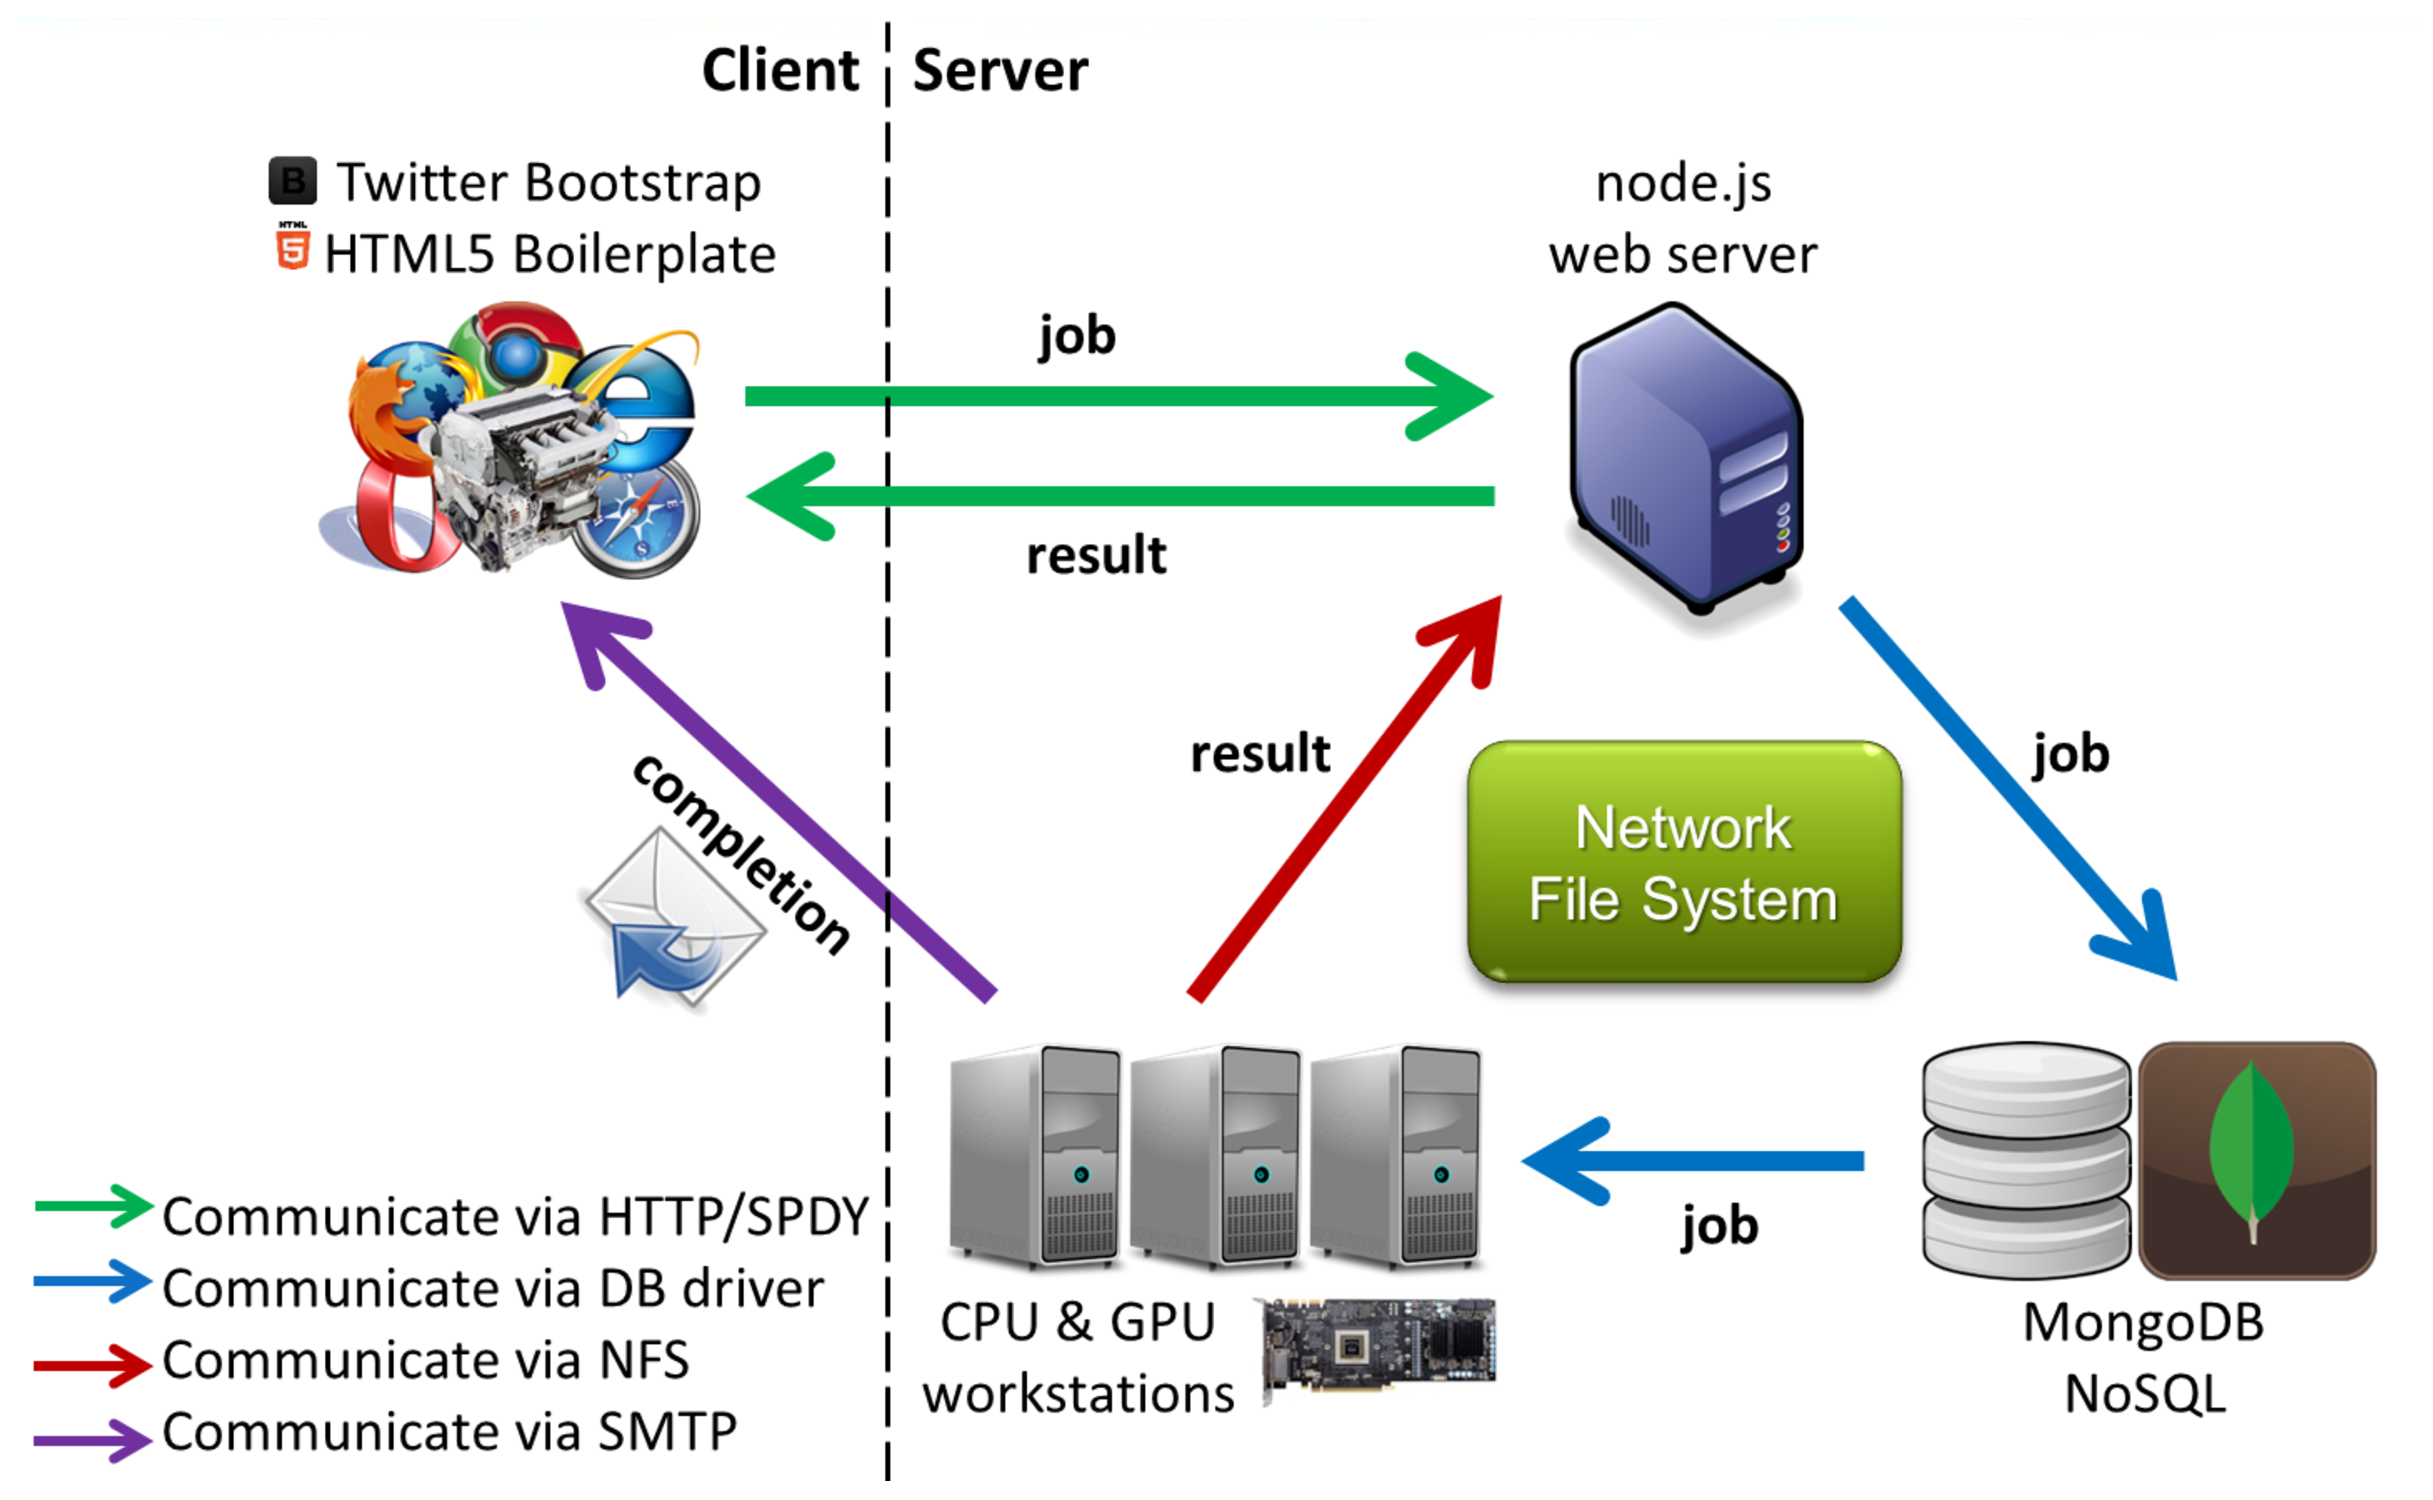
\includegraphics[width=4in]{Architecture.eps}
\end{center}
\caption{
{\bf The overall architecture of istar.} There are five major components: a web site, a web server, a database management system, several workstations, and a network file system.
}
\label{Architecture}
\end{figure}

\begin{figure}[!ht]
\begin{center}
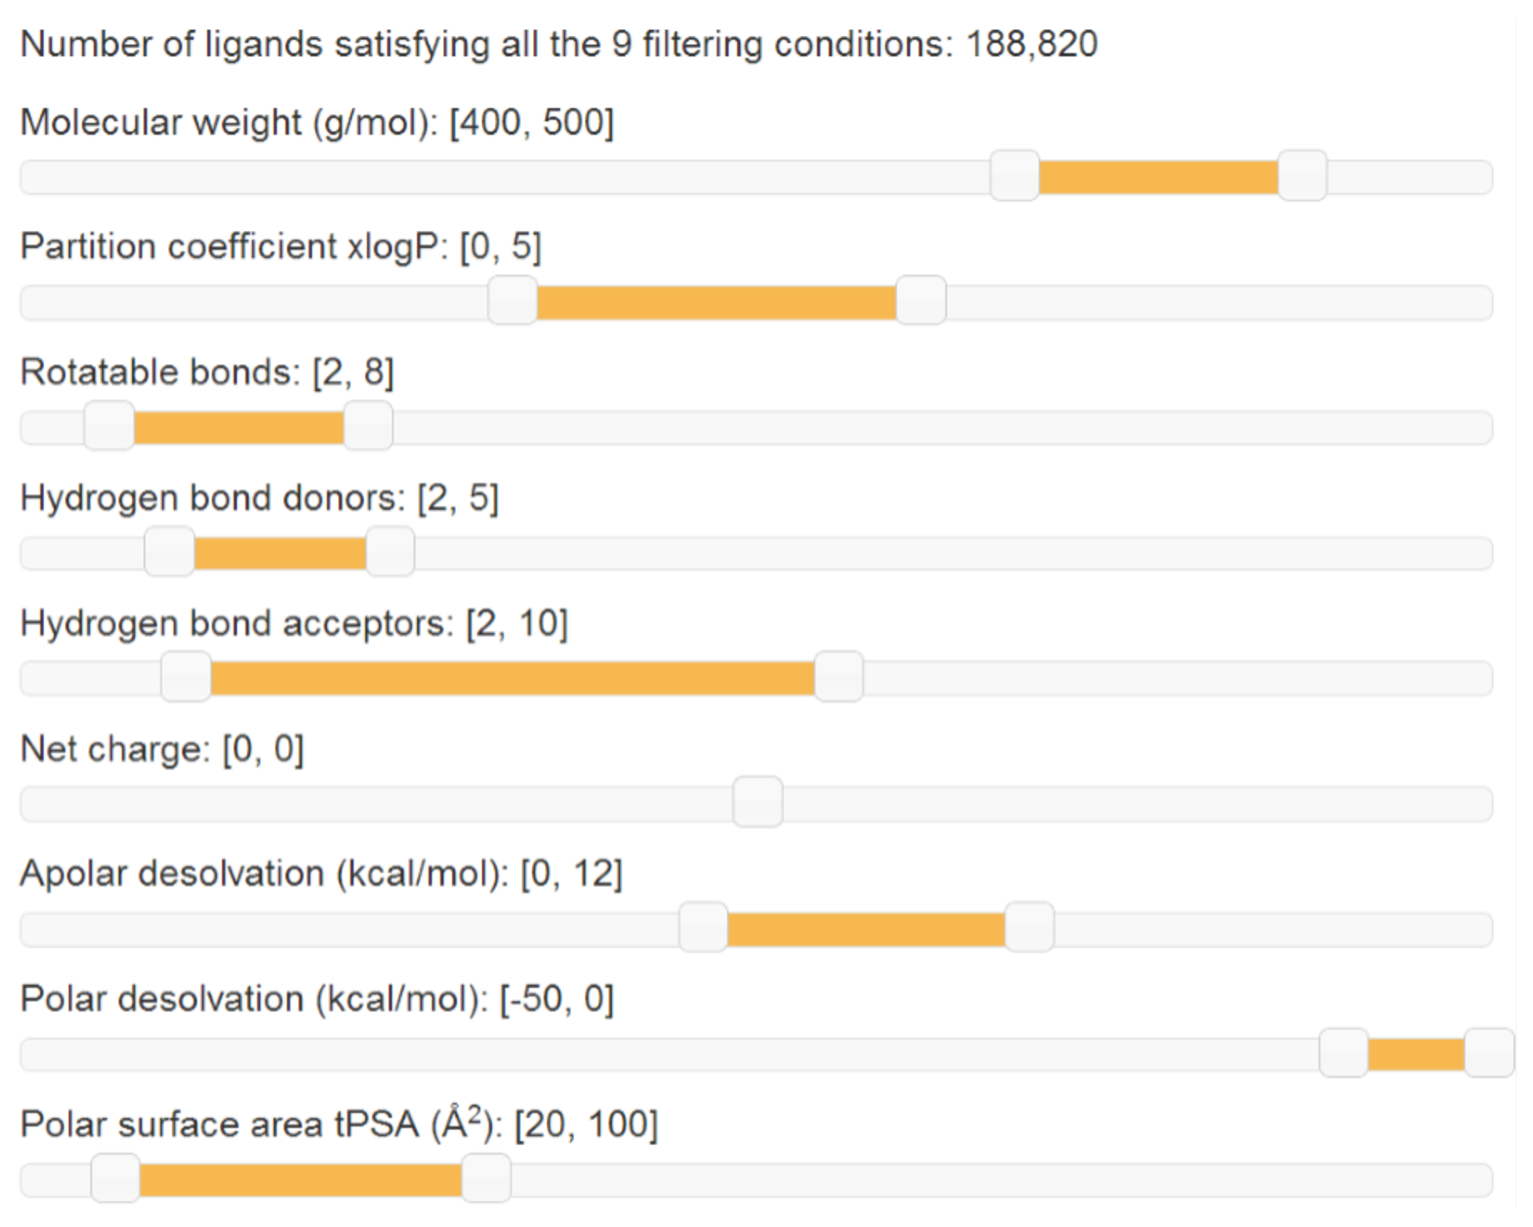
\includegraphics[width=4in]{Slider.eps}
\end{center}
\caption{
{\bf istar supports filtering ligands with molecular properties in a fine-grained manner and previewing the number of ligands to dock in real time.} Users can move the nine sliders to filter ligands in the form of closed intervals.
}
\label{Slider}
\end{figure}

\begin{figure}[!ht]
\begin{center}
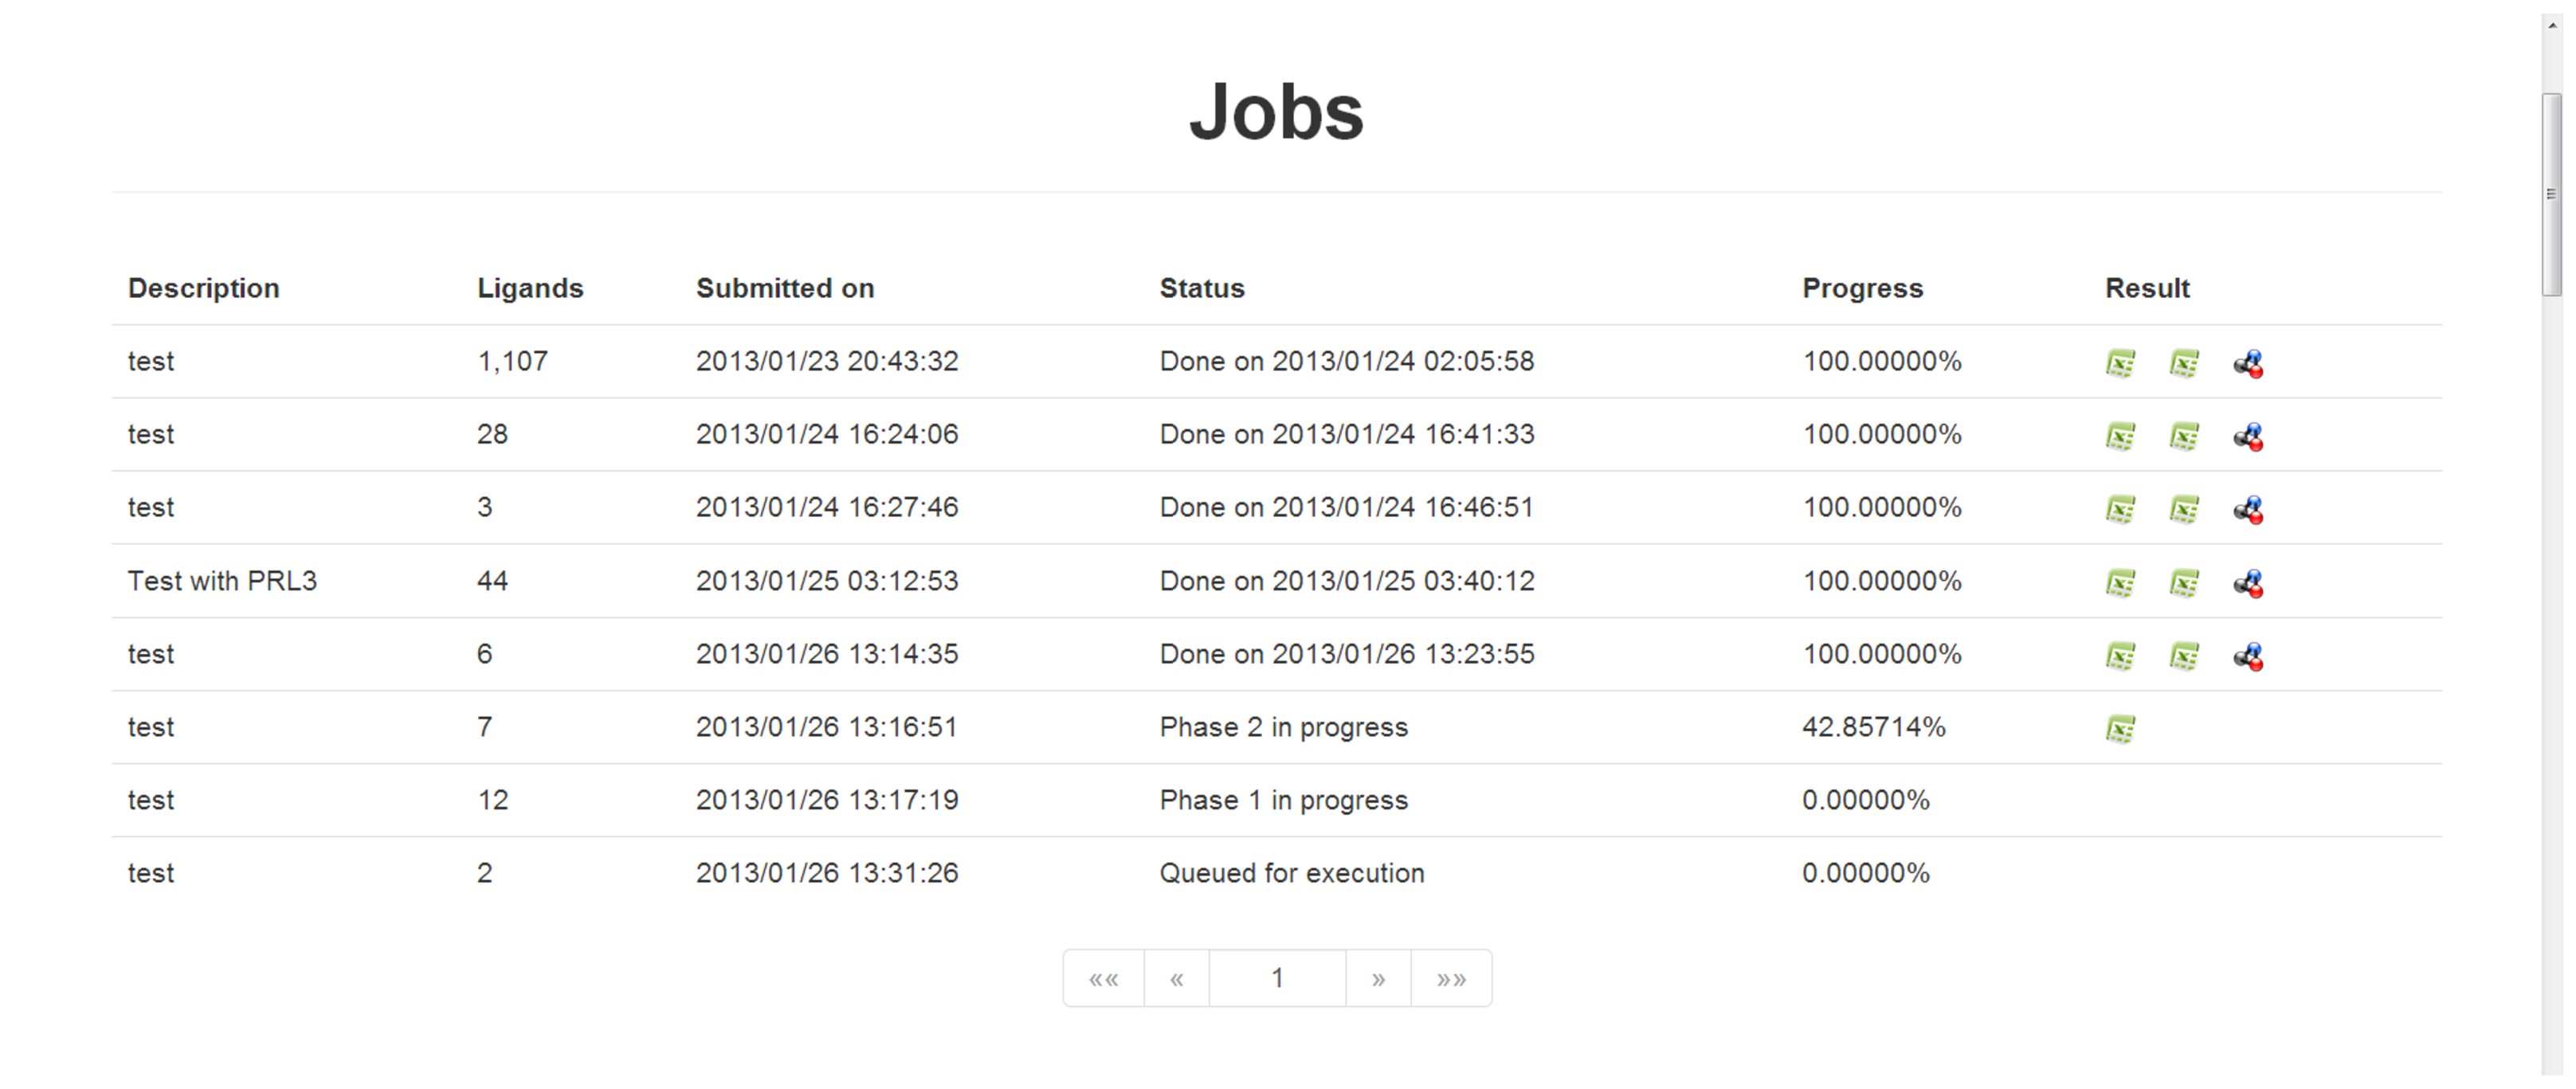
\includegraphics[width=4in]{Progress.eps}
\end{center}
\caption{
{\bf istar supports monitoring job progress in real time.} Users can thus have a rough estimation in advance of how long the jobs will take and when the jobs will complete.
}
\label{Progress}
\end{figure}

\begin{figure}[!ht]
\begin{center}
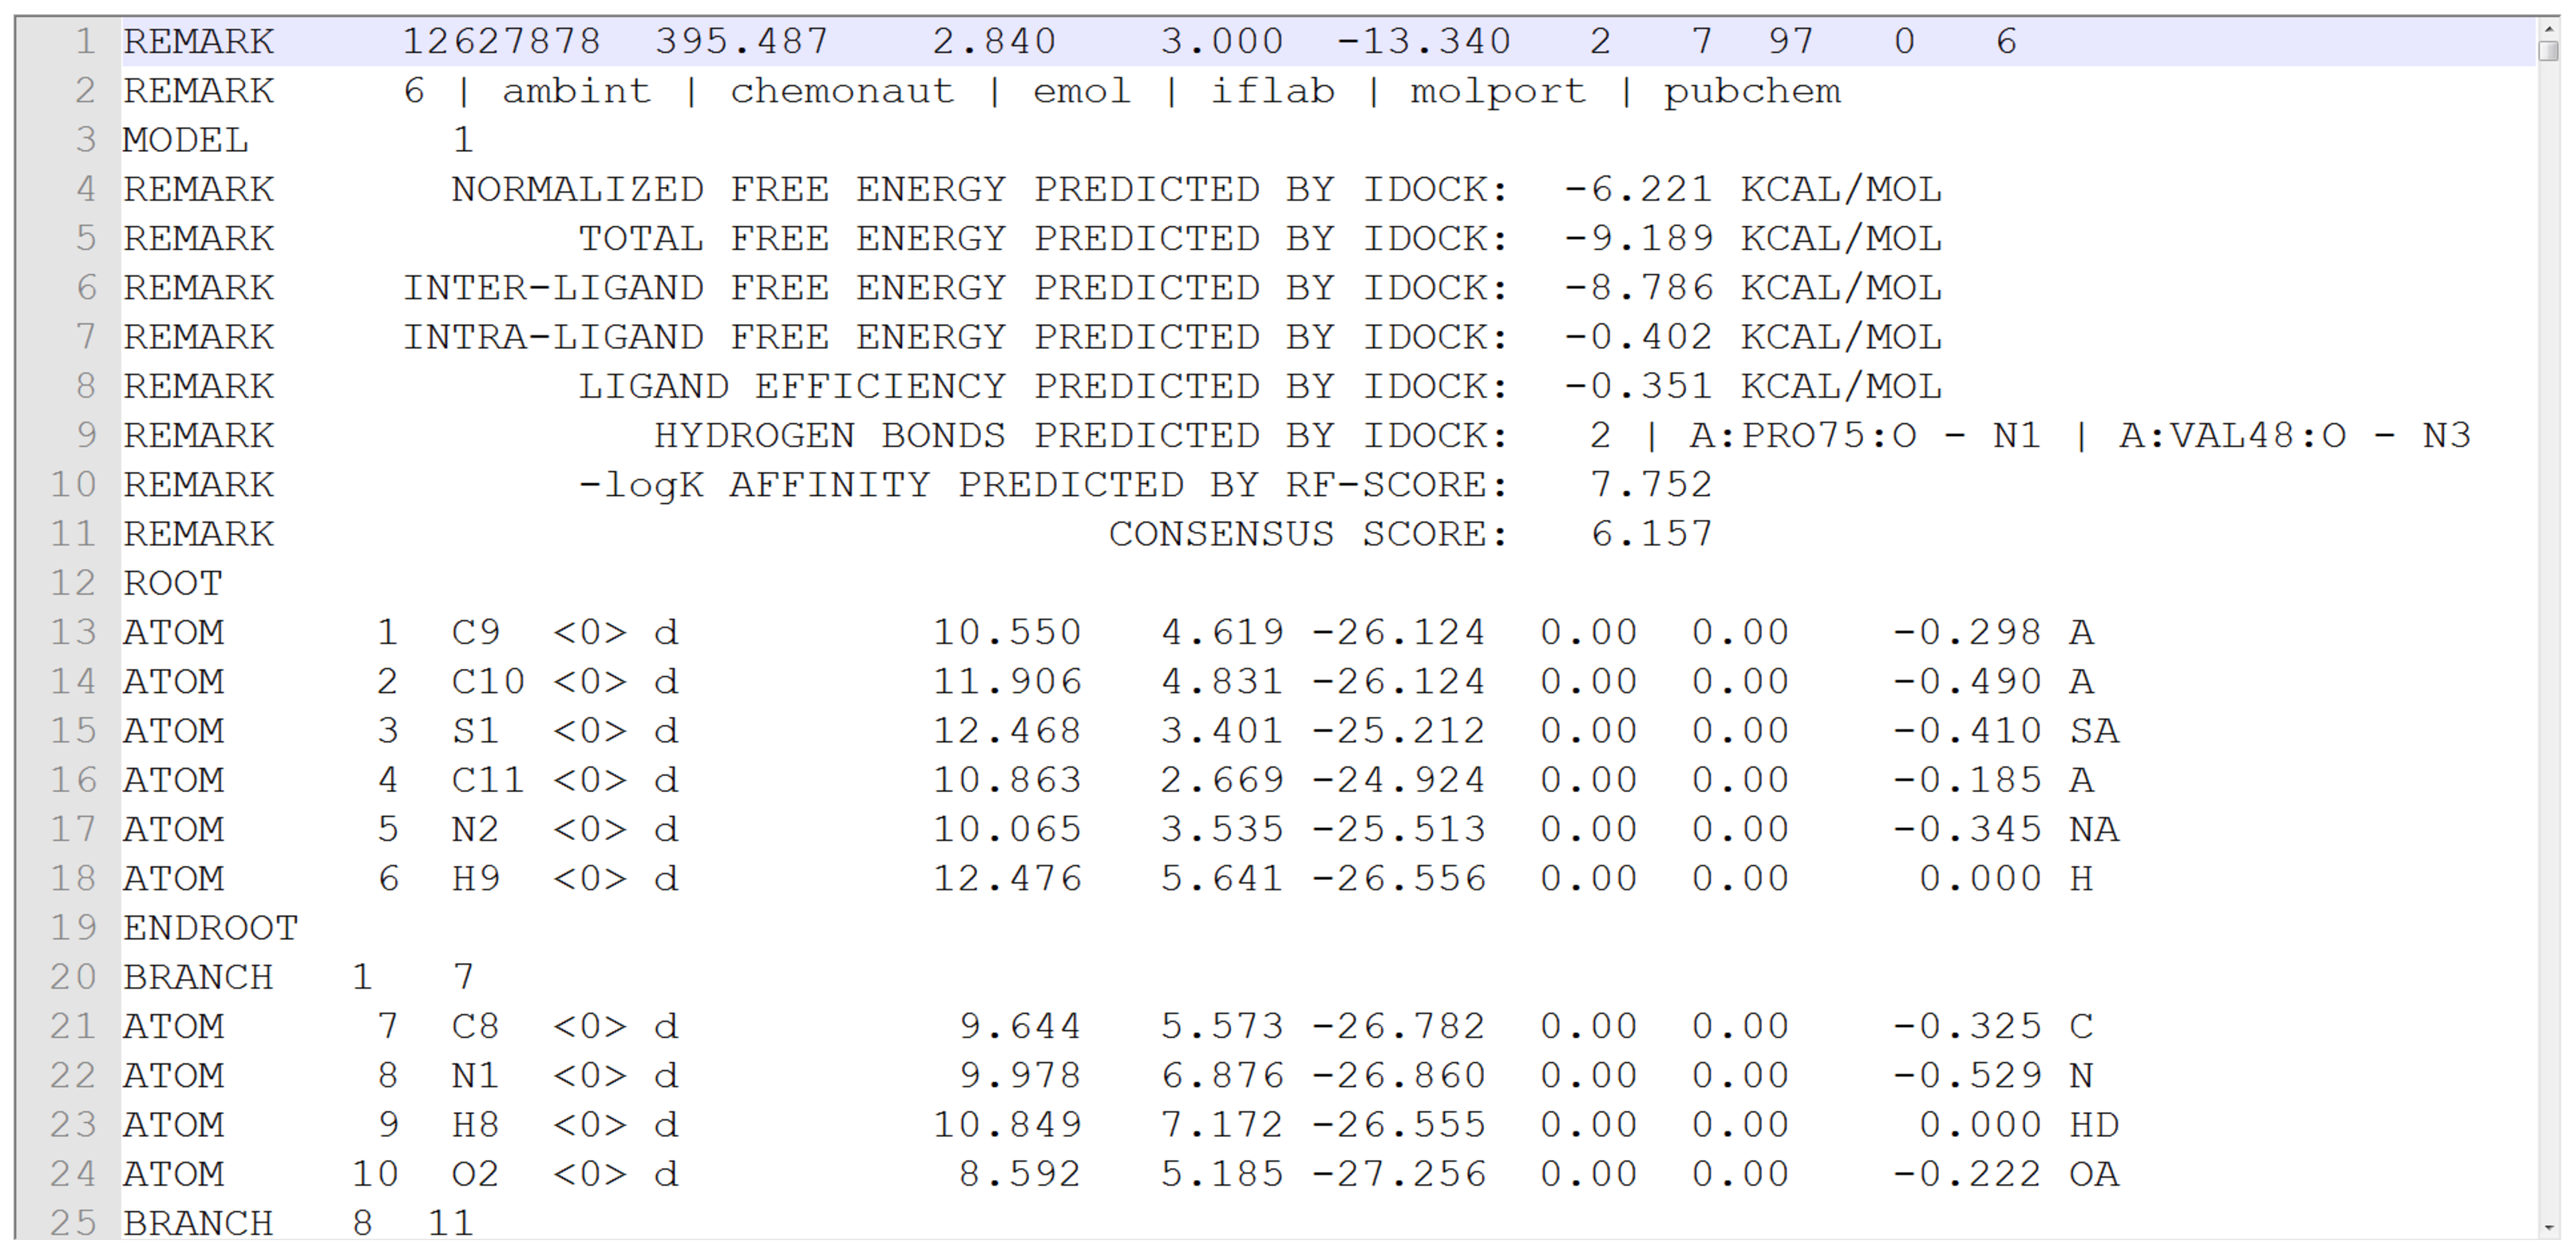
\includegraphics[width=4in]{OutputPDBQT.eps}
\end{center}
\caption{
{\bf istar writes verbose output to file in PDBQT format.} The REMARK lines describe the ZINC ID, molecular properties and suppliers of a ligand. For each predicted conformation, the REMARK lines also describe the free energy and ligand efficiency predicted by idock, putative hydrogen bonds, binding affinity predicted by RF-Score, and consensus score in $pK_d$ or $pK_i$ unit. Columns 71 to 76 of the ATOM lines describe per-atom free energy predicted by idock.
}
\label{OutputPDBQT}
\end{figure}

\begin{figure}[!ht]
\begin{center}
\includegraphics[width=4in]{PDBbind2012Correlations.eps}
\end{center}
\caption{
{\bf Pairwise correlations of experimental binding affinity and predicted binding affinity by RF-Score, AutoDock Vina and idock on the PDBbind v2012 refined set ($N$ = 2,897).} Along the diagonal from top left to bottom right are the histogram distributions of experimental binding affinity and predicted binding affinity by RF-Score, AutoDock Vina, and idock, respectively. Values are in $pK_d$ or $pK_i$ unit. $R_p$ = 0.965, $R_s$ = 0.966, $RMSE$ = 0.60, $SD$ = 0.60 for RF-Score, $R_p$ = 0.466, $R_s$ = 0.464, $RMSE$ = 2.29, $SD$ = 2.21 for Vina, and $R_p$ = 0.451, $R_s$ = 0.453, $RMSE$ = 2.28, $SD$ = 2.25 for idock.
}
\label{PDBbind2012Correlations}
\end{figure}

\begin{figure}[!ht]
\begin{center}
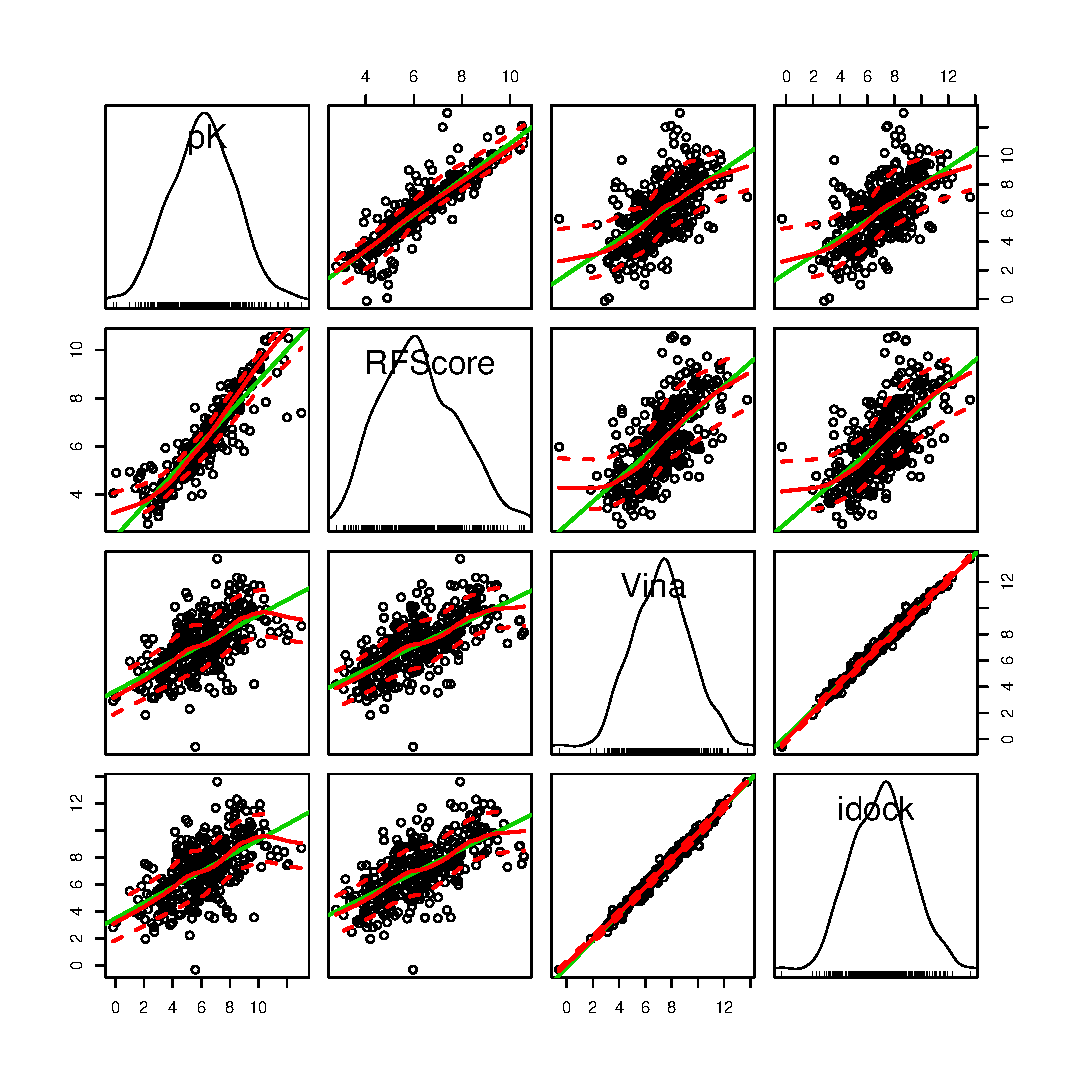
\includegraphics[width=4in]{CSAR2010Correlations.eps}
\end{center}
\caption{
{\bf Pairwise correlations of experimental binding affinity and predicted binding affinity by RF-Score, AutoDock Vina and idock on the CSAR NRC HiQ Set 24Sept2010 ($N$ = 343).} Along the diagonal from top left to bottom right are the histogram distributions of experimental binding affinities and predicted binding affinities by RF-Score, AutoDock Vina, and idock, respectively. Values are in $pK_d$ or $pK_i$ unit. $R_p$ = 0.899, $R_s$ = 0.926, $RMSE$ = 1.05, $SD$ = 1.05 for RF-Score, $R_p$ = 0.595, $R_s$ = 0.611, $RMSE$ = 2.26, $SD$ = 1.98 for Vina, and $R_p$ = 0.597, $R_s$ = 0.613, $RMSE$ = 2.17, $SD$ = 1.97 for idock.
}
\label{CSAR2010Correlations}
\end{figure}

\begin{figure}[!ht]
\begin{center}
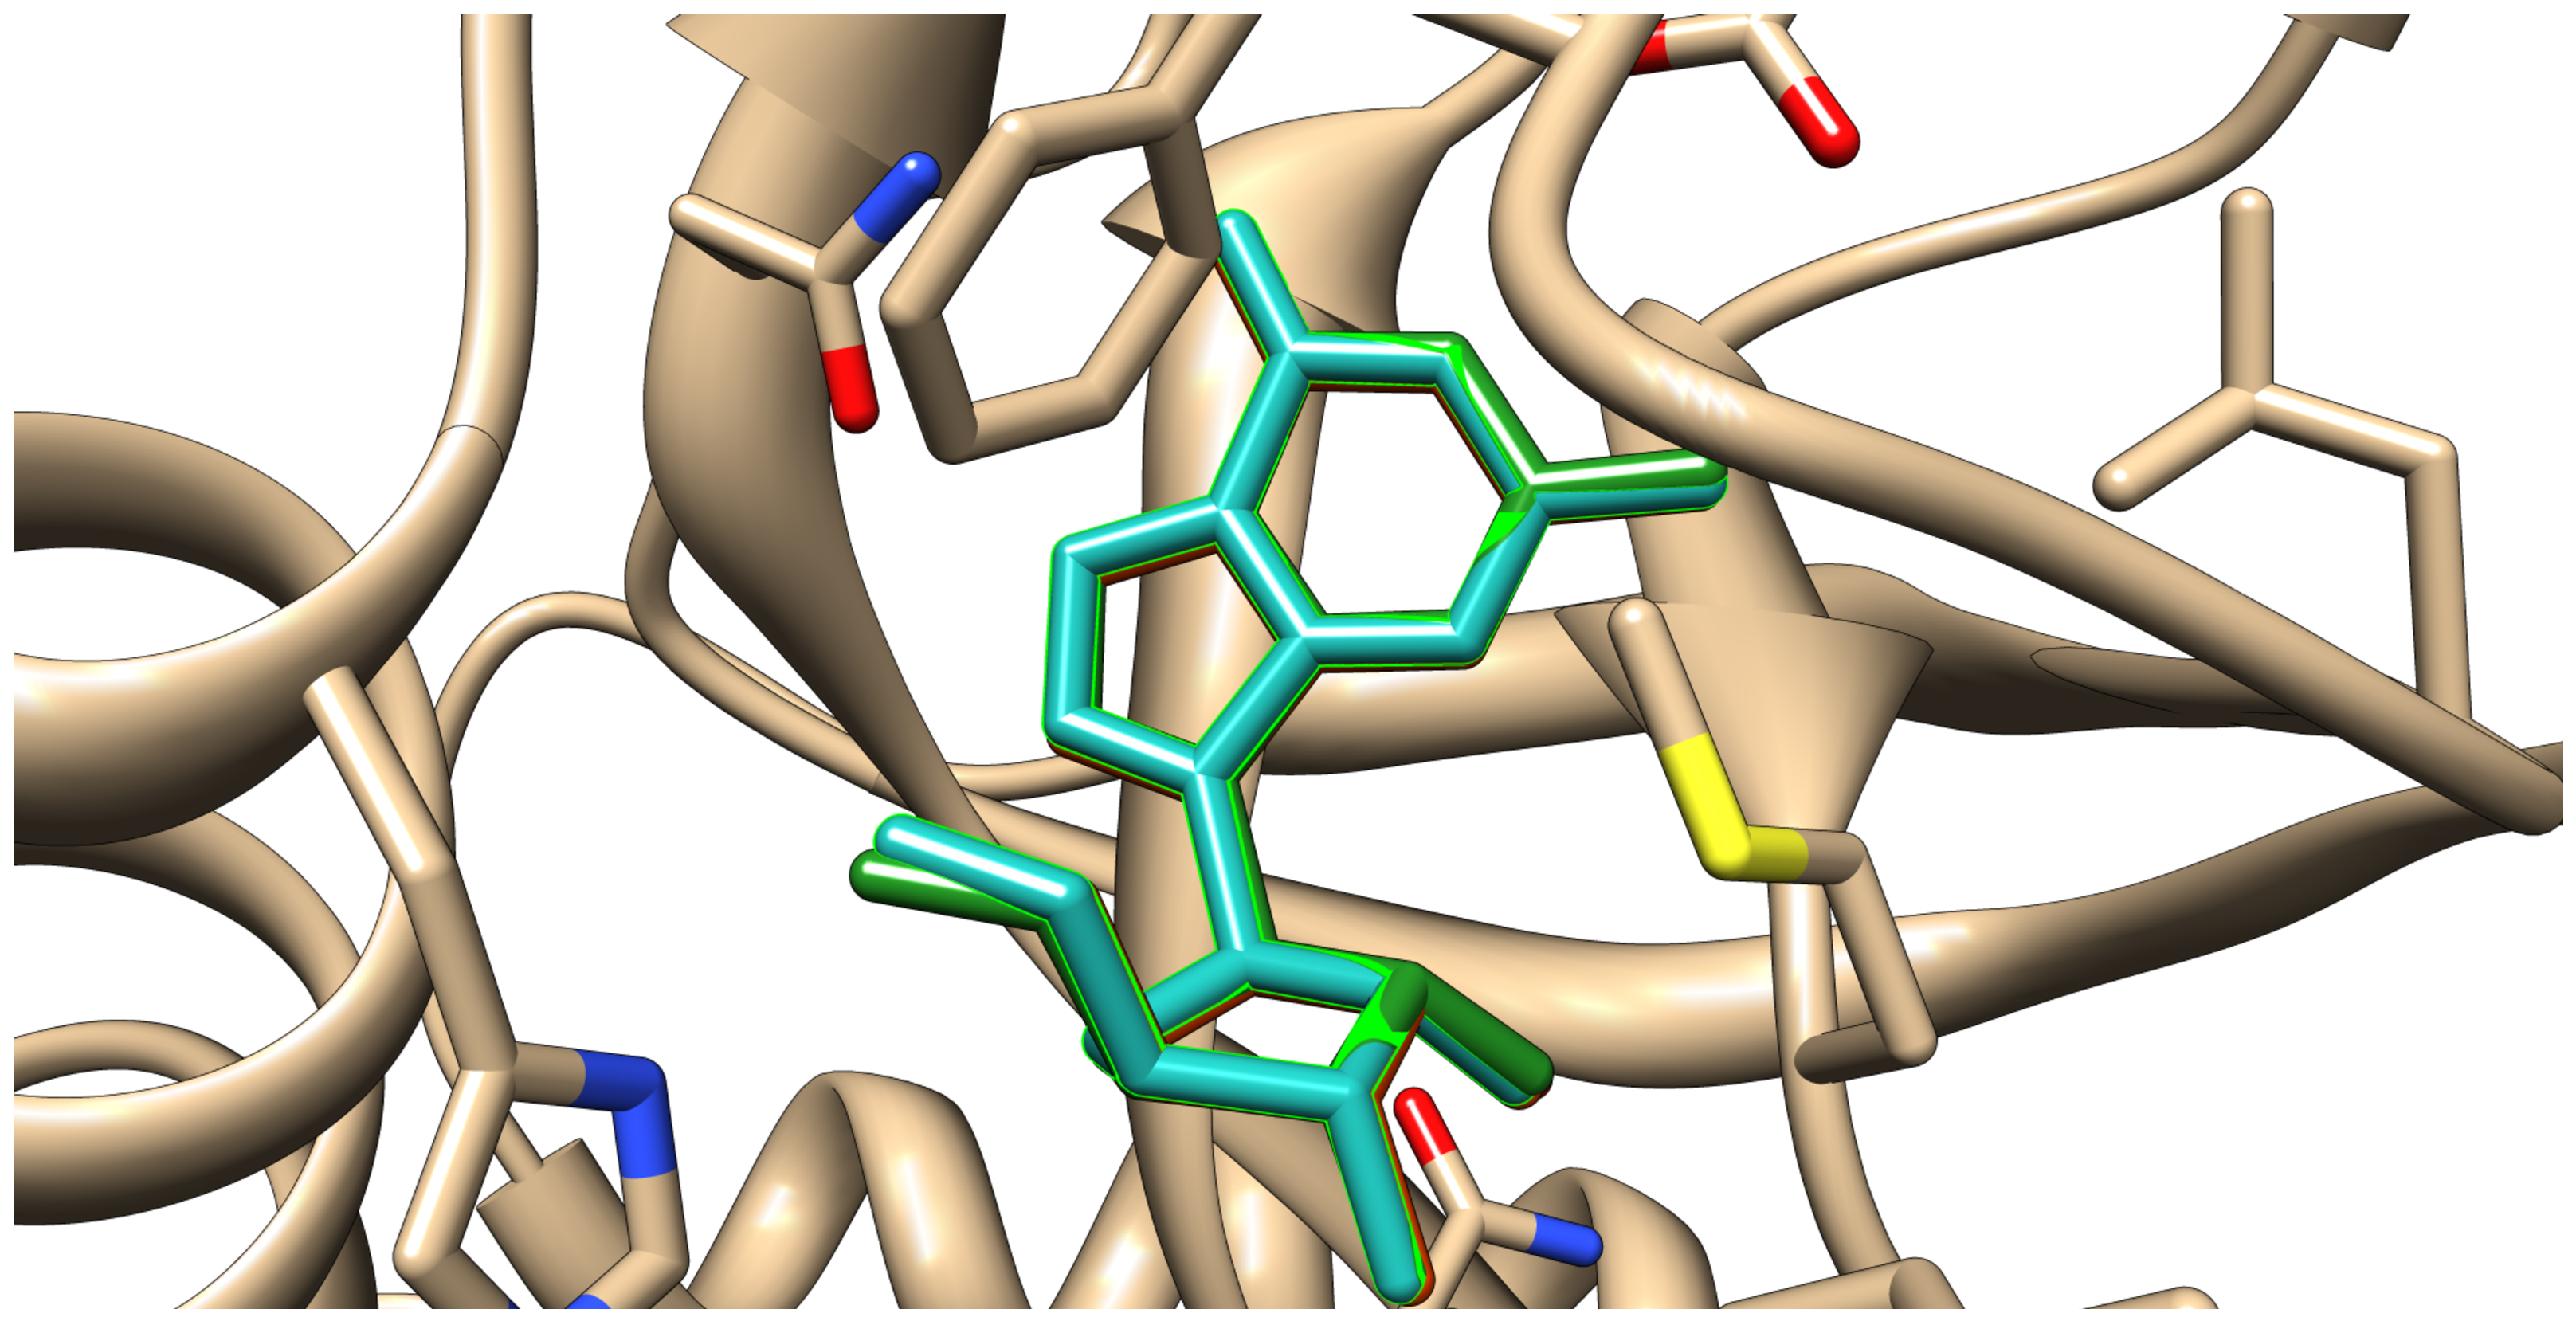
\includegraphics[width=4in]{Redocking1B8N.eps}
\end{center}
\caption{
{\bf Redocking result of PDB ID 1B8N.} The protein target is purine nucleoside phosphorylase. The crystal ligand conformation is rendered in green. The conformation predicted by Vina is rendered in red. The conformation predicted by idock is rendered in blue. The same color scheme applies to the subsequent three redocking cases. $RMSD$ = 0.139\AA\ for Vina, and $RMSD$ = 0.127\AA\ for idock. Both programs managed to predict a conformation close enough to the crystal one.
}
\label{Redocking1B8N}
\end{figure}

\begin{figure}[!ht]
\begin{center}
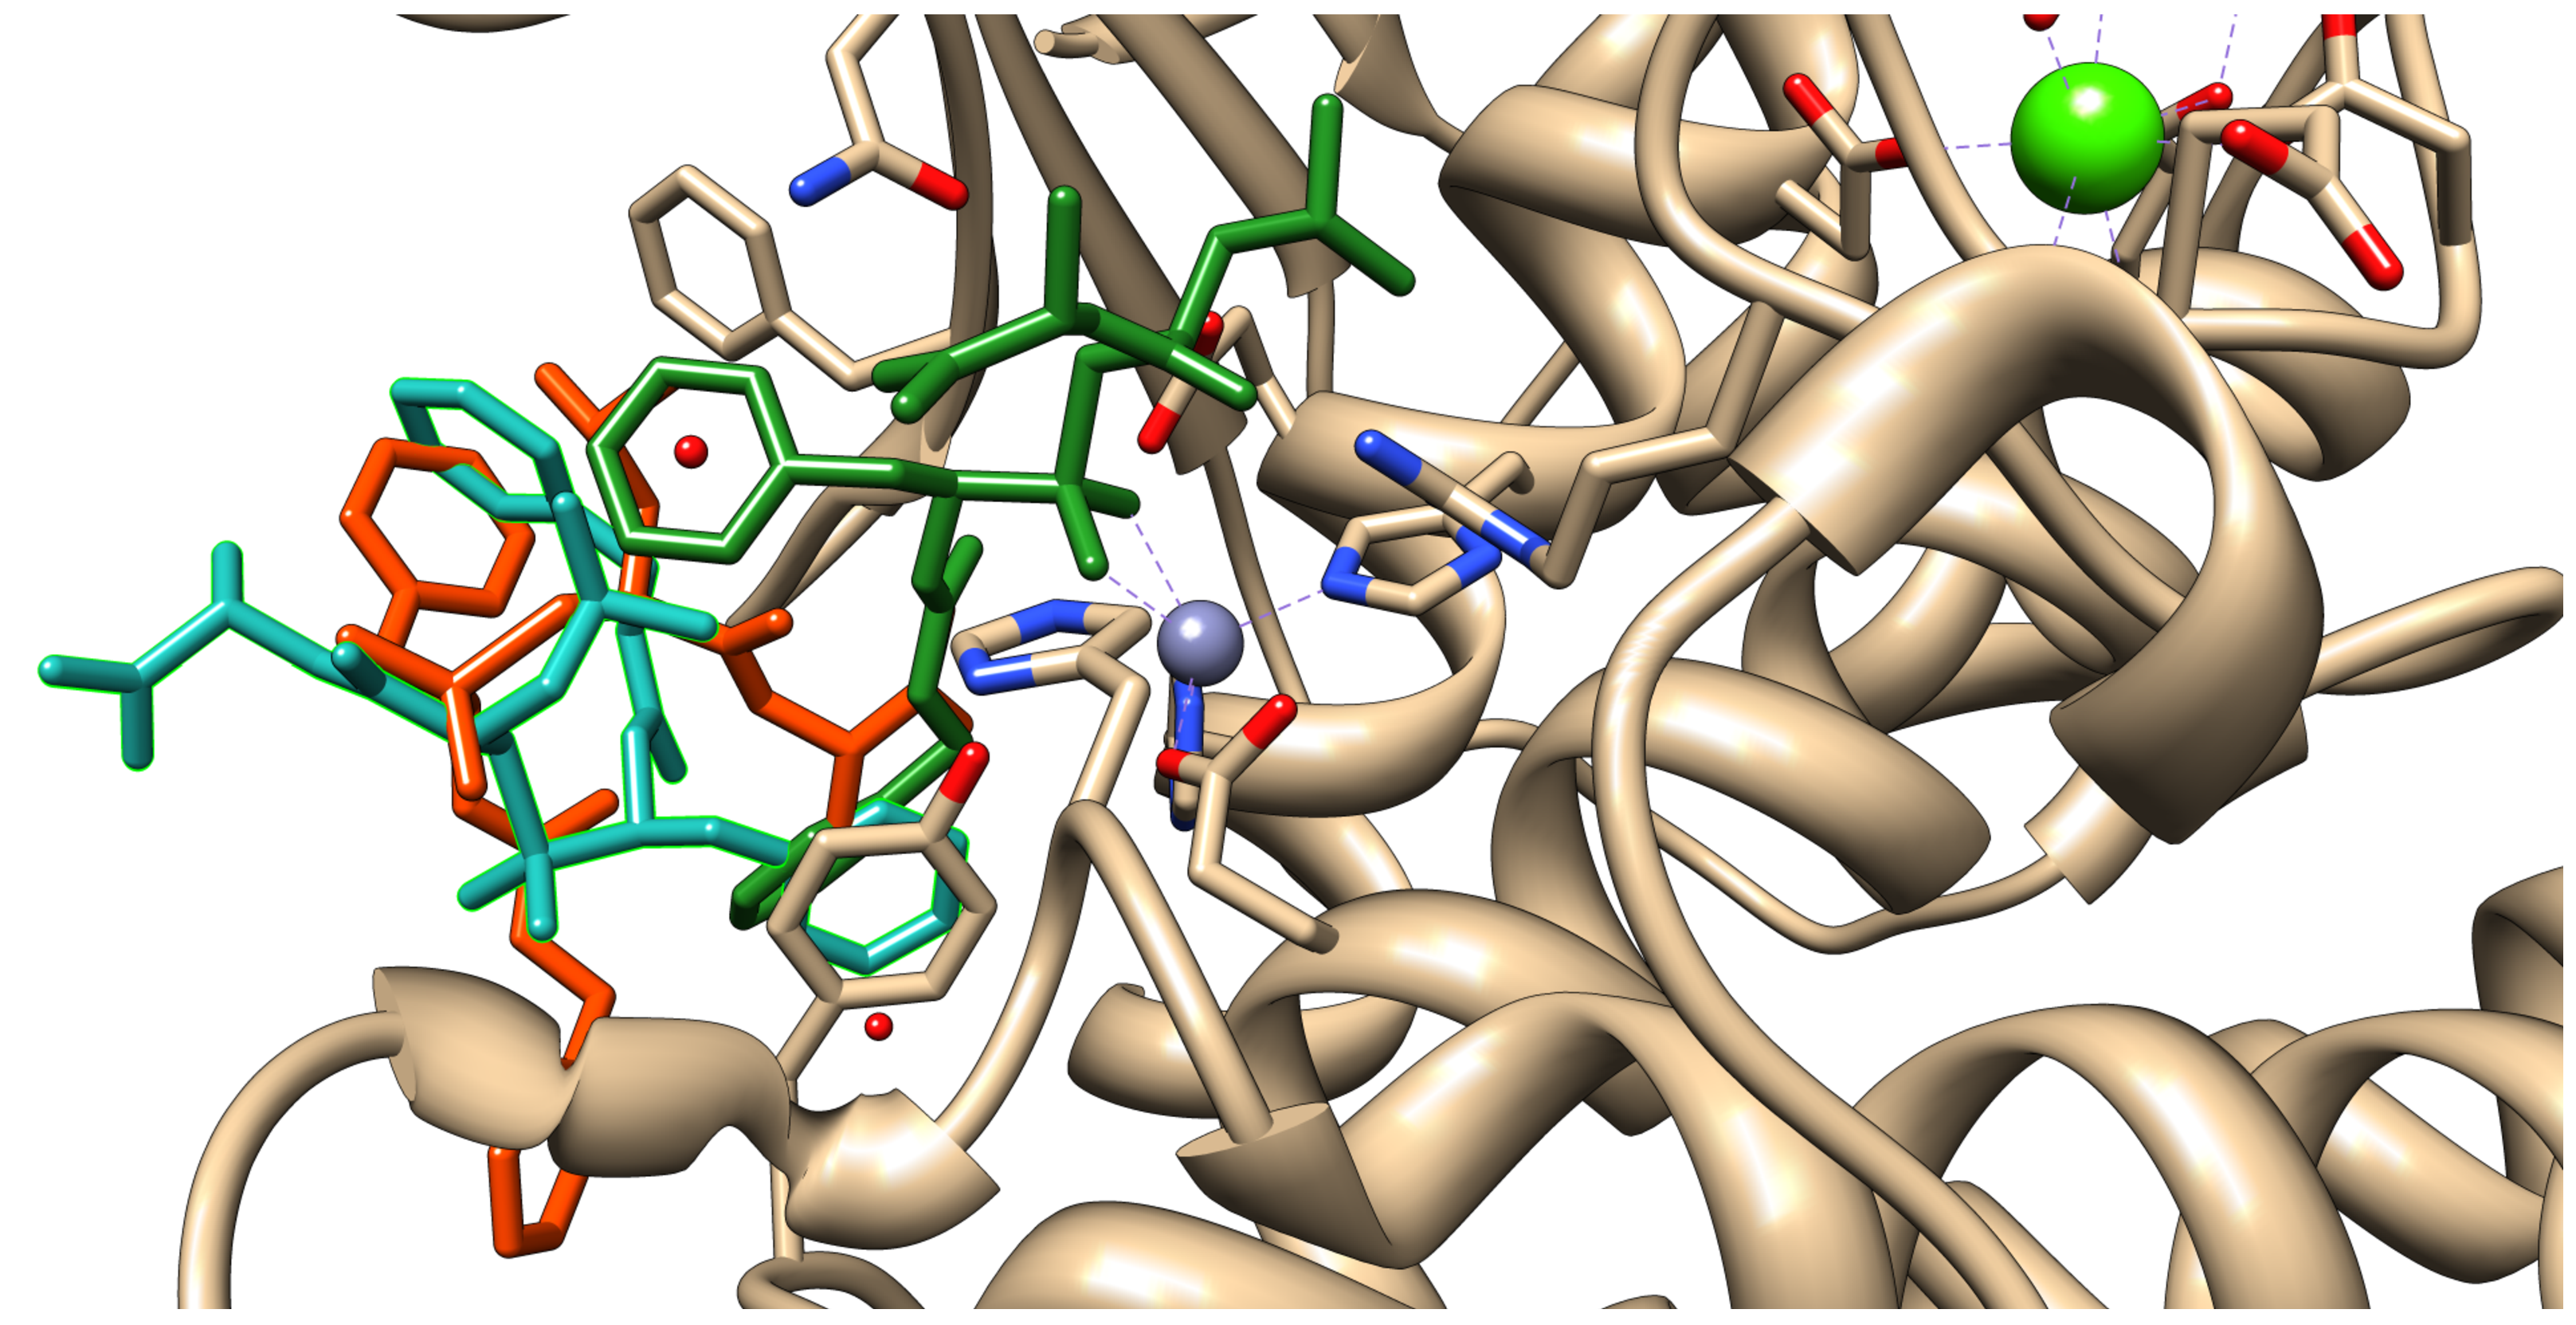
\includegraphics[width=4in]{Redocking4TMN.eps}
\end{center}
\caption{
{\bf Redocking result of PDB ID 4TMN.} The protein target is thermolysin. $RMSD$ = 8.401\AA\ for Vina, and $RMSD$ = 9.909\AA\ for idock. Both programs failed to predict a conformation close enough to the crystal one, probably due to the presence of a zinc ion in the binding site.
}
\label{Redocking4TMN}
\end{figure}

\begin{figure}[!ht]
\begin{center}
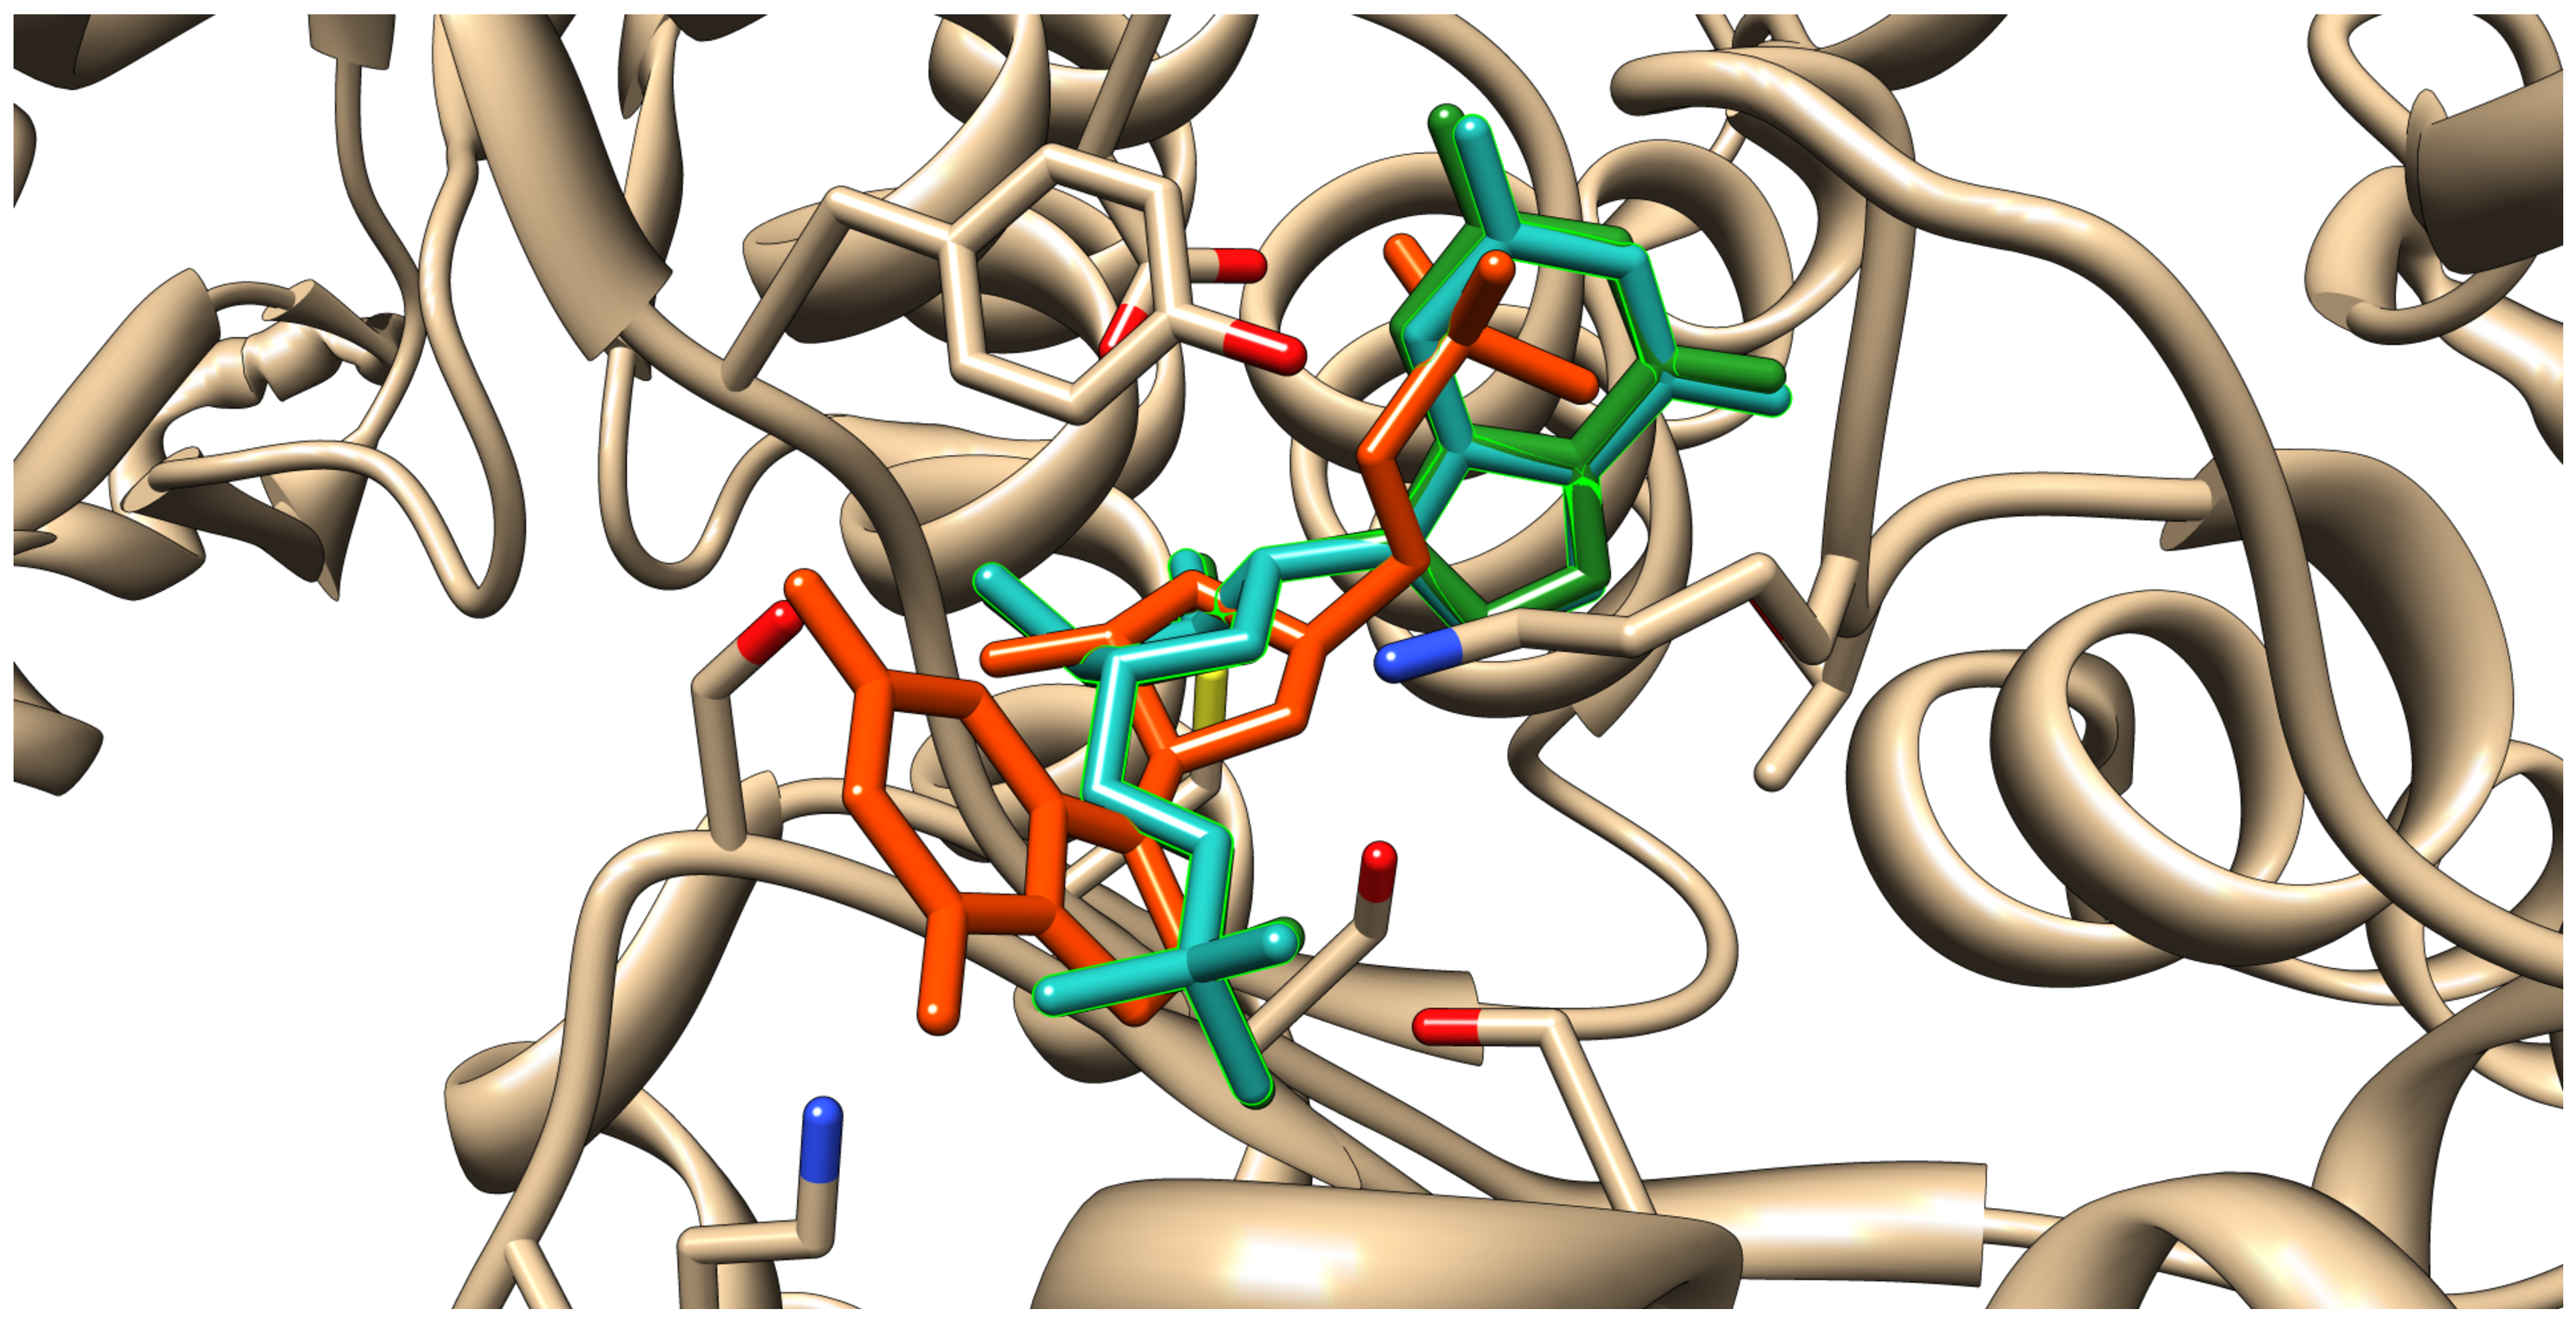
\includegraphics[width=4in]{Redocking1PKX.eps}
\end{center}
\caption{
{\bf Redocking result of PDB ID 1PKX.} The protein target is bifunctional purine biosynthesis protein PURH. $RMSD$ = 7.059\AA\ for Vina, and $RMSD$ = 0.214\AA\ for idock. idock managed to predict a conformation close enough to the crystal one but AutoDock Vina failed.
}
\label{Redocking1PKX}
\end{figure}

\begin{figure}[!ht]
\begin{center}
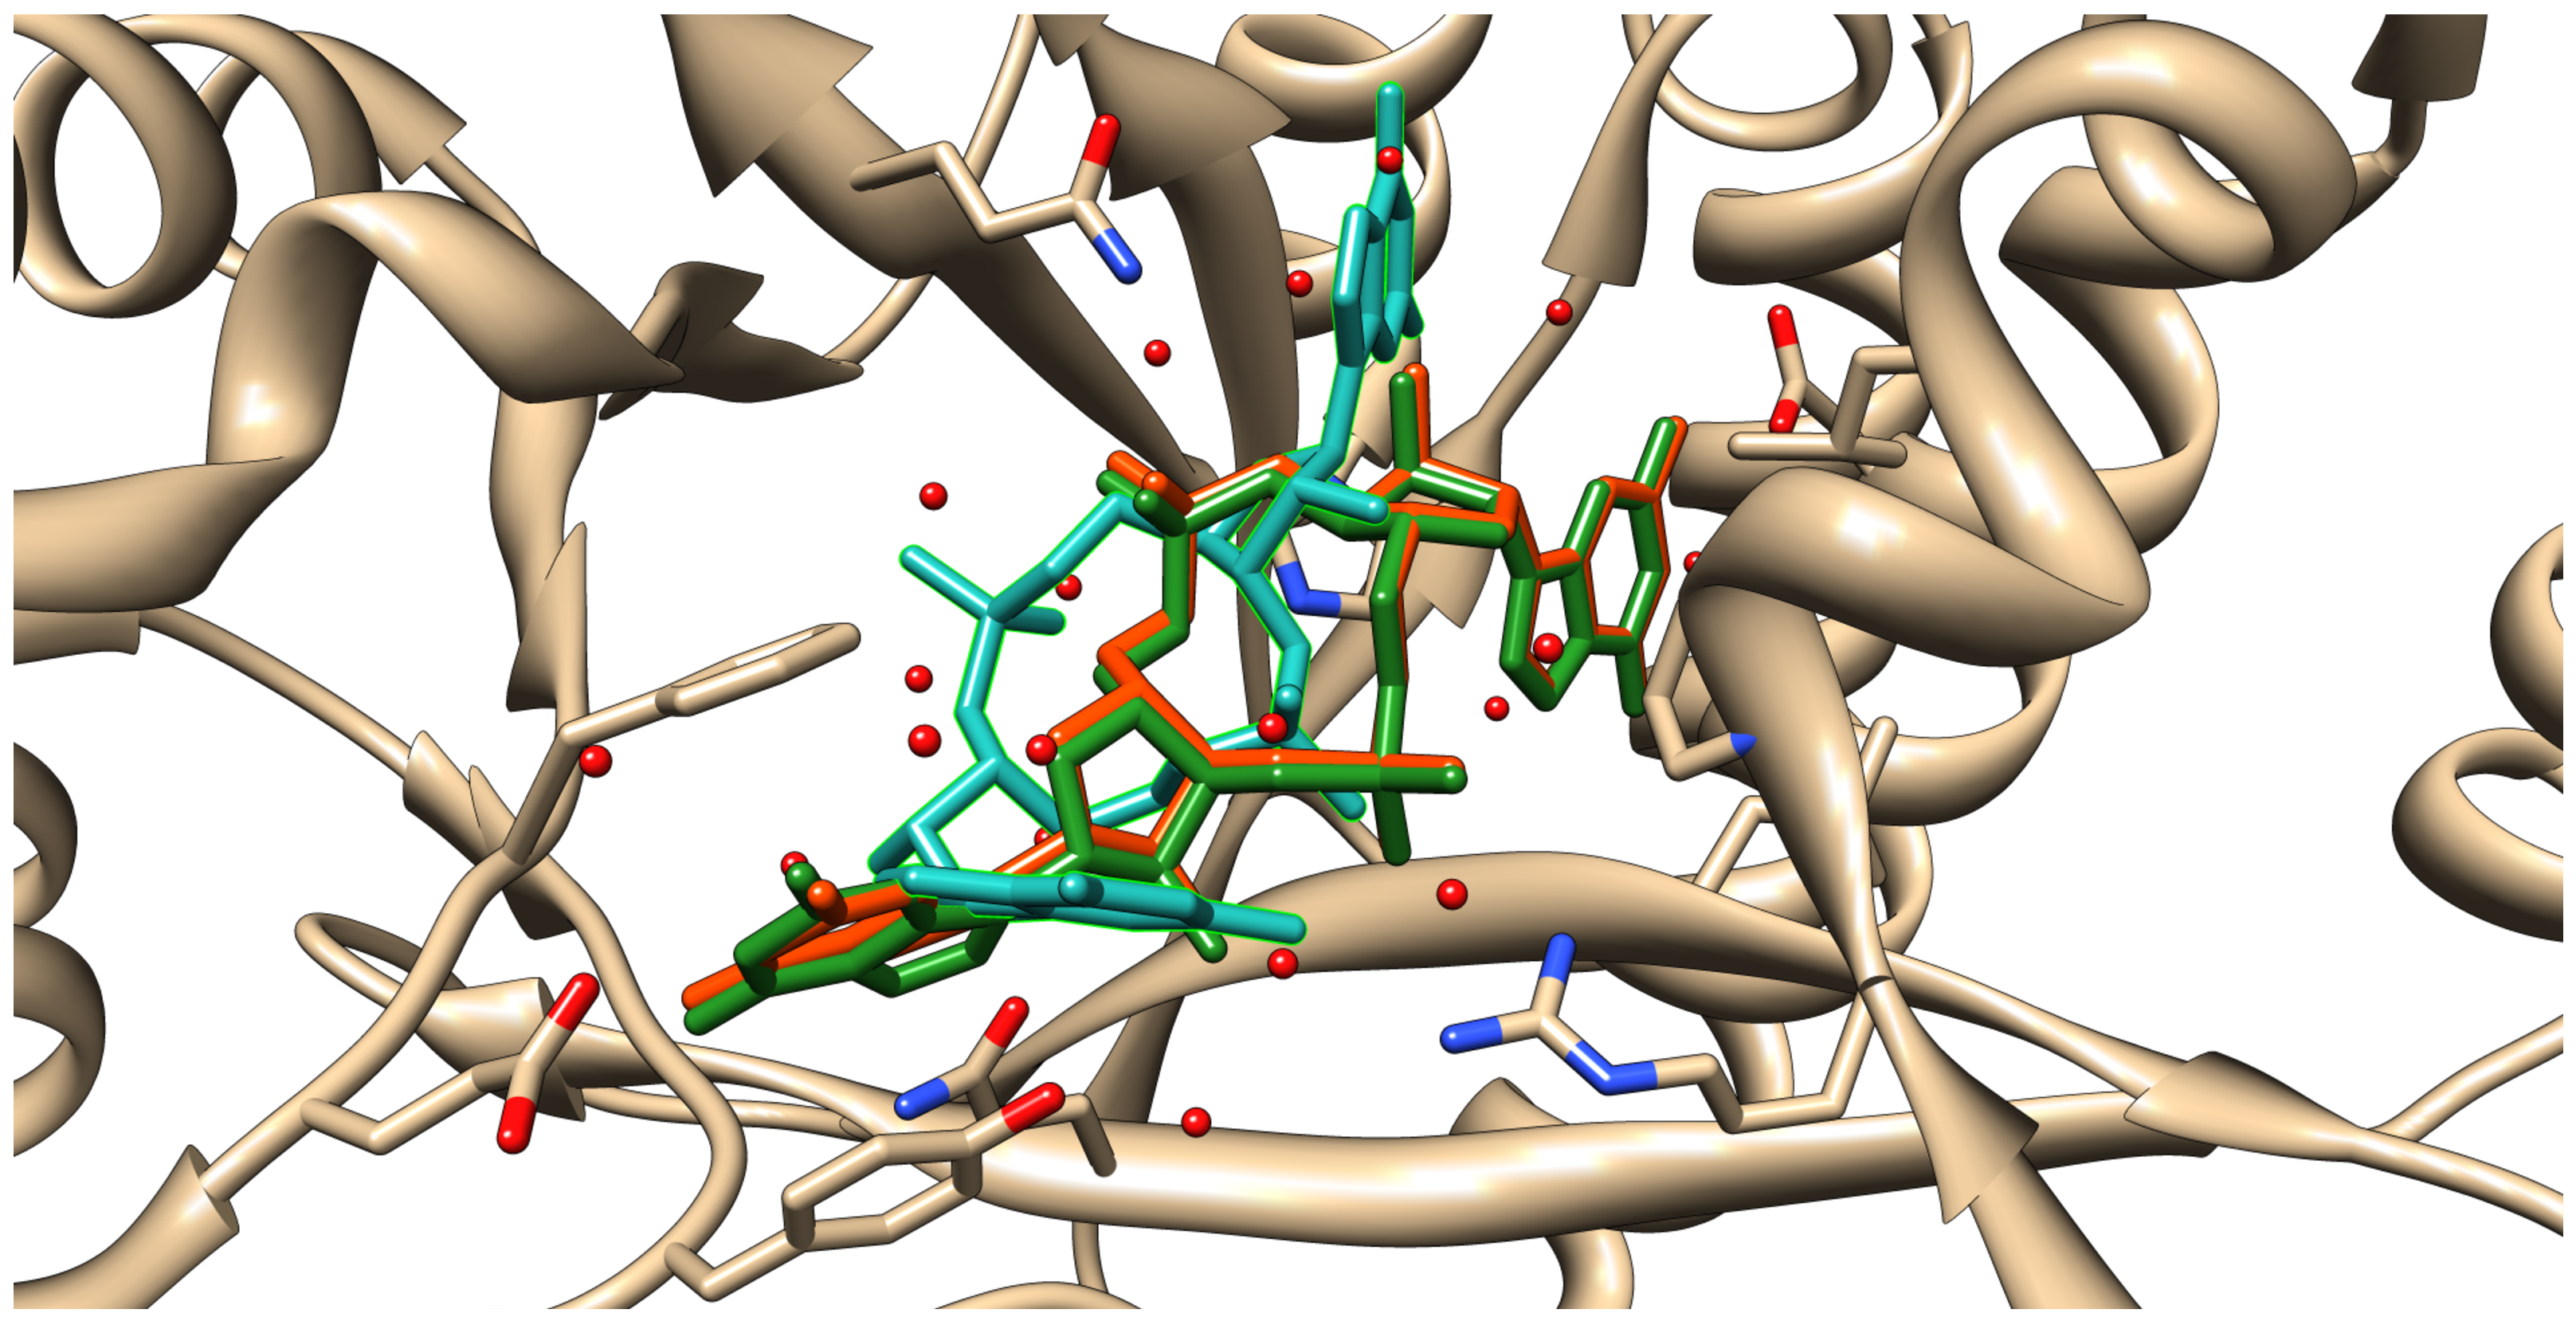
\includegraphics[width=4in]{Redocking3HV8.eps}
\end{center}
\caption{
{\bf Redocking result of PDB ID 3HV8.} The protein target is FimX. $RMSD$ = 0.290\AA\ for Vina, and $RMSD$ = 10.232\AA\ for idock. AutoDock Vina managed to predict a conformation close enough to the crystal one but idock failed.
}
\label{Redocking3HV8}
\end{figure}

\begin{figure}[!ht]
\begin{center}
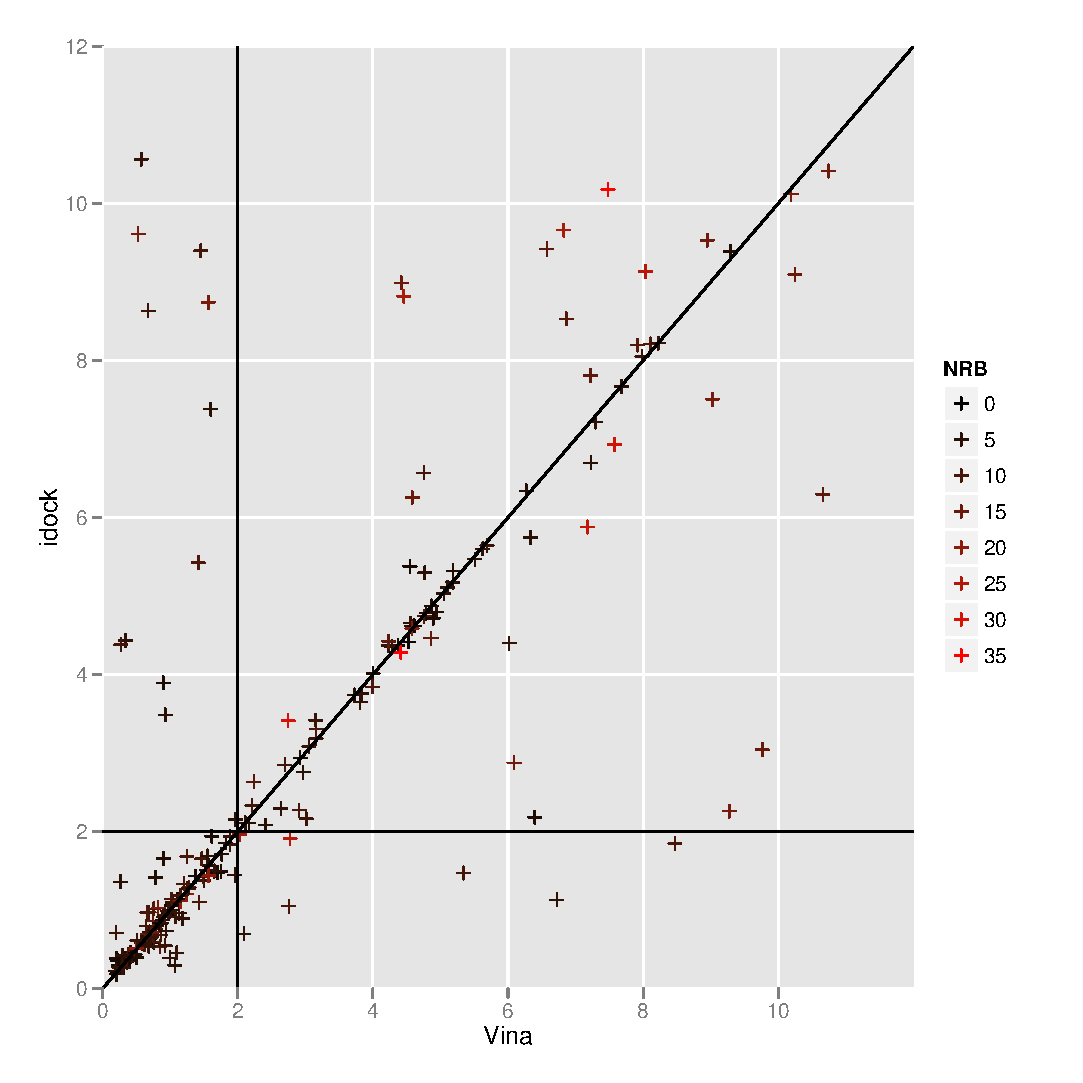
\includegraphics[width=4in]{VinaConf1RMSD-idockConf1RMSD.eps}
\end{center}
\caption{
{\bf $RMSD_1$ of the predicted ligand conformation from the crystal one, showing the values for idock and AutoDock Vina. The color encodes the number of active rotatable bonds (NRB).} $RMSD_1$ refers to the $RMSD$ value between the crystal conformation and the docked conformation with the highest predicted binding affinity. Very often the $RMSD$ of 2.0 \AA\ is regarded as the positive control for correct bound structure prediction.
}
\label{VinaConf1RMSD-idockConf1RMSD}
\end{figure}

\begin{figure}[!ht]
\begin{center}
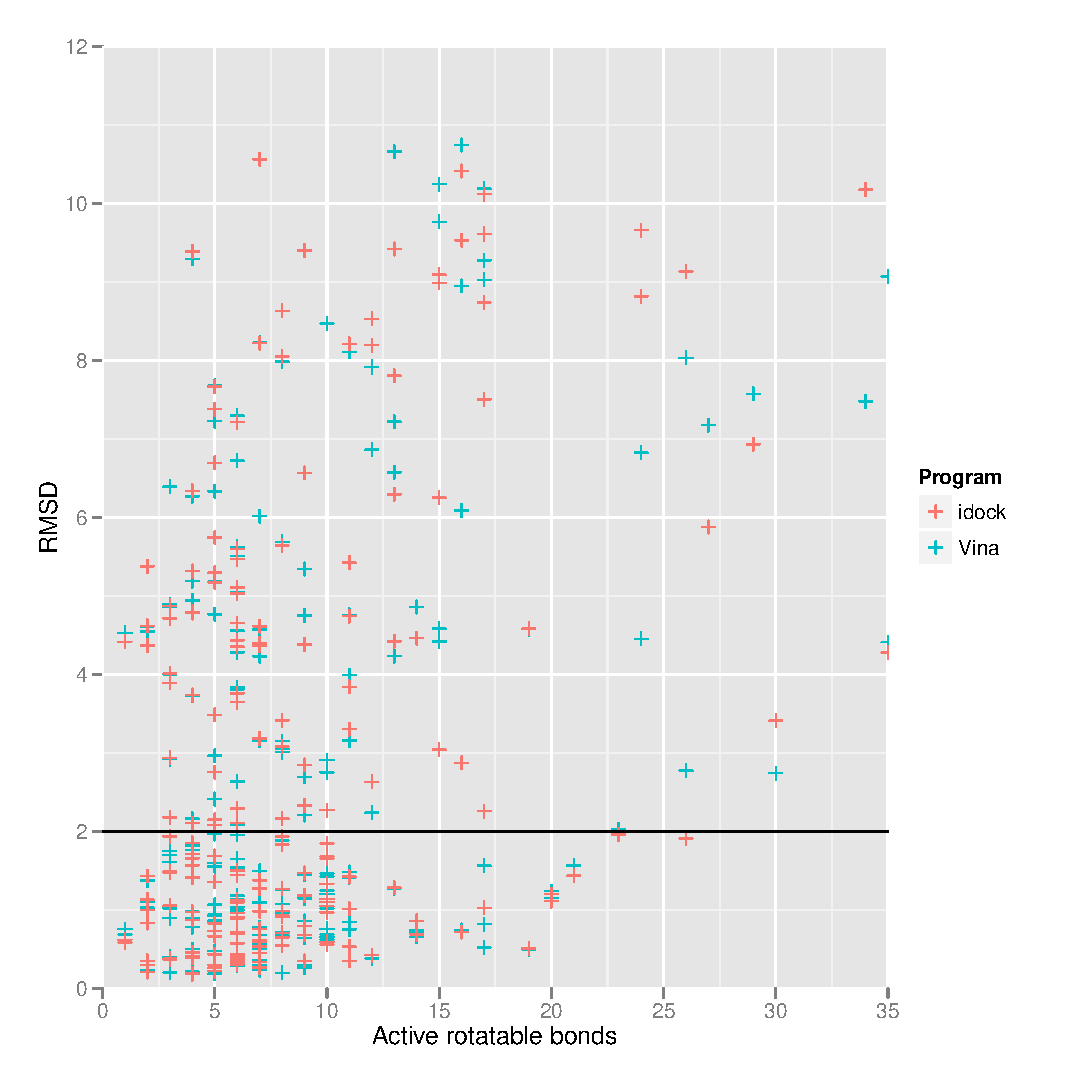
\includegraphics[width=4in]{NRB-RMSD.eps}
\end{center}
\caption{
{\bf $RMSD_1$ of the predicted ligand conformation from the crystal one. Abscissa shows the number of active rotatable bonds (NRB).} $RMSD_1$ refers to the $RMSD$ value between the crystal conformation and the docked conformation with the highest predicted binding affinity. Very often the $RMSD$ of 2.0 \AA\ is regarded as the positive control for correct bound structure prediction.
}
\label{NRB-RMSD}
\end{figure}

\begin{figure}[!ht]
\begin{center}
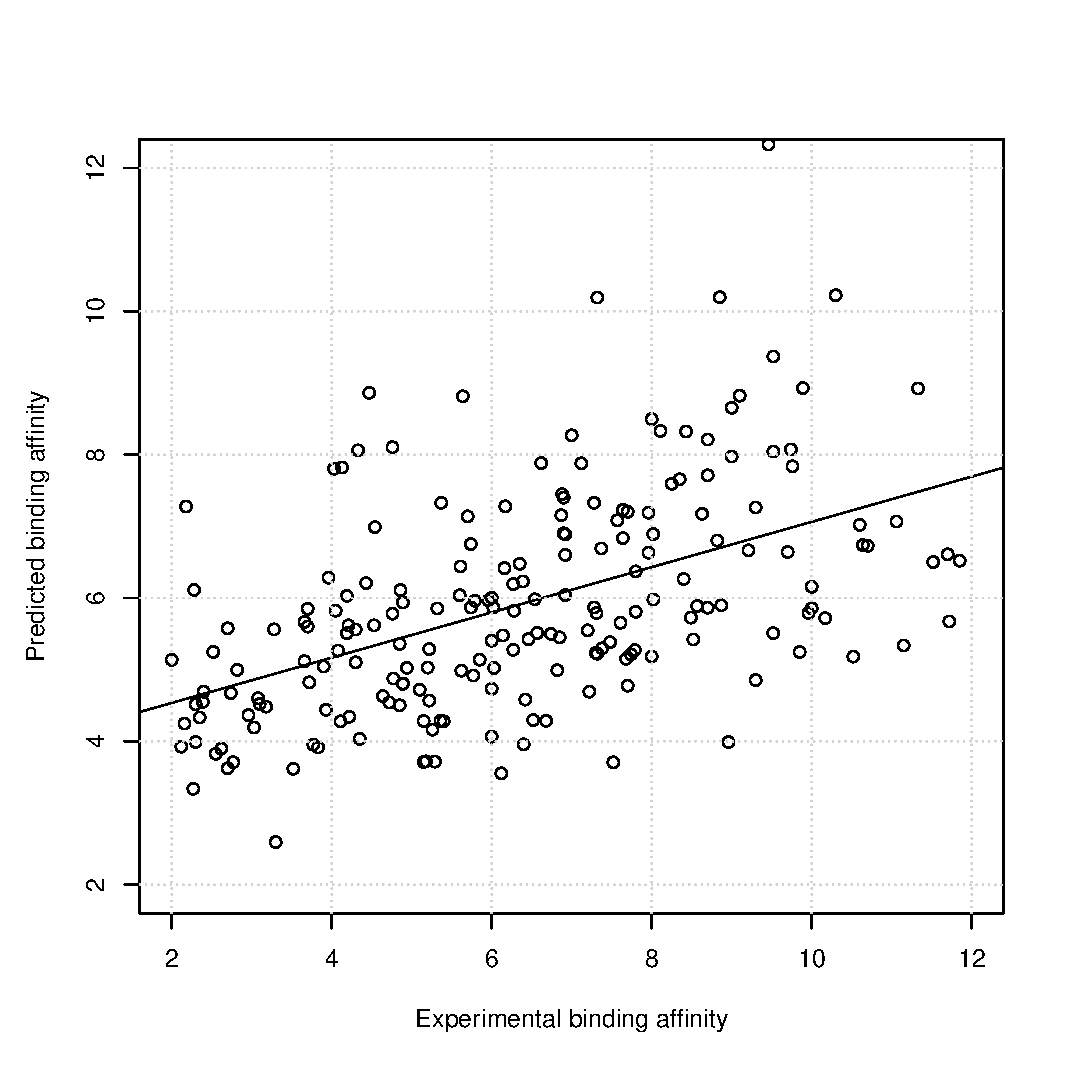
\includegraphics[width=4in]{pK-idockConf1idock.eps}
\end{center}
\caption{
{\bf Scatter plot of predicted binding affinity of docked pose against experimental binding affinity on PDBbind v2012 core set ($N$ = 201).} $R_p$ = 0.502, $R_s$ = 0.530, $RMSE$ = 2.15, $SD$ = 2.11.
}
\label{pK-idockConf1idock}
\end{figure}

\begin{figure}[!ht]
\begin{center}
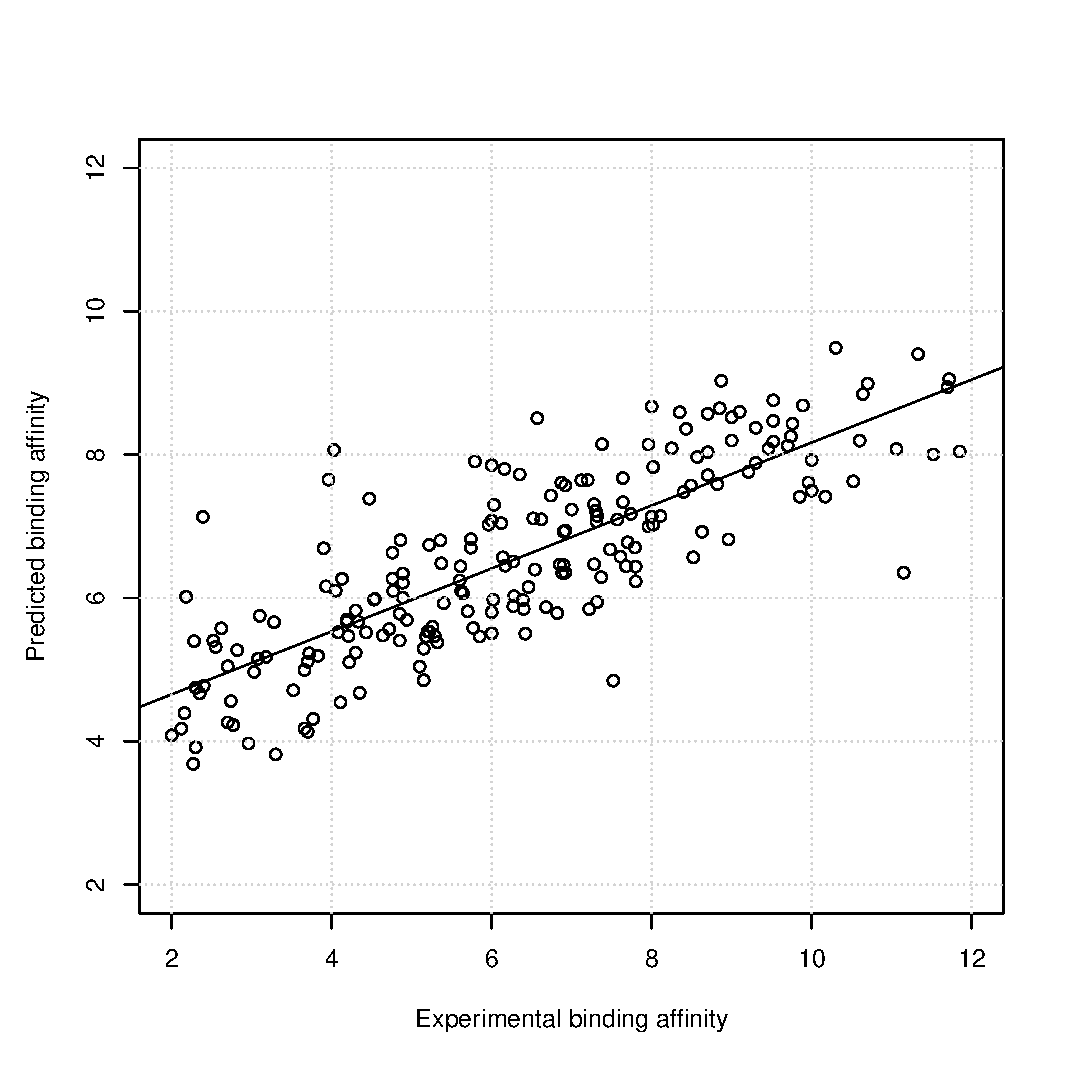
\includegraphics[width=4in]{pK-idockConfsRFScoreMax.eps}
\end{center}
\caption{
{\bf Scatter plot of predicted binding affinity of docked pose against experimental binding affinity on PDBbind v2012 core set ($N$ = 201).} $R_p$ = 0.815, $R_s$ = 0.817, $RMSE$ = 1.57, $SD$ = 1.55.
}
\label{pK-idockConfsRFScoreMax}
\end{figure}

\begin{figure}[!ht]
\begin{center}
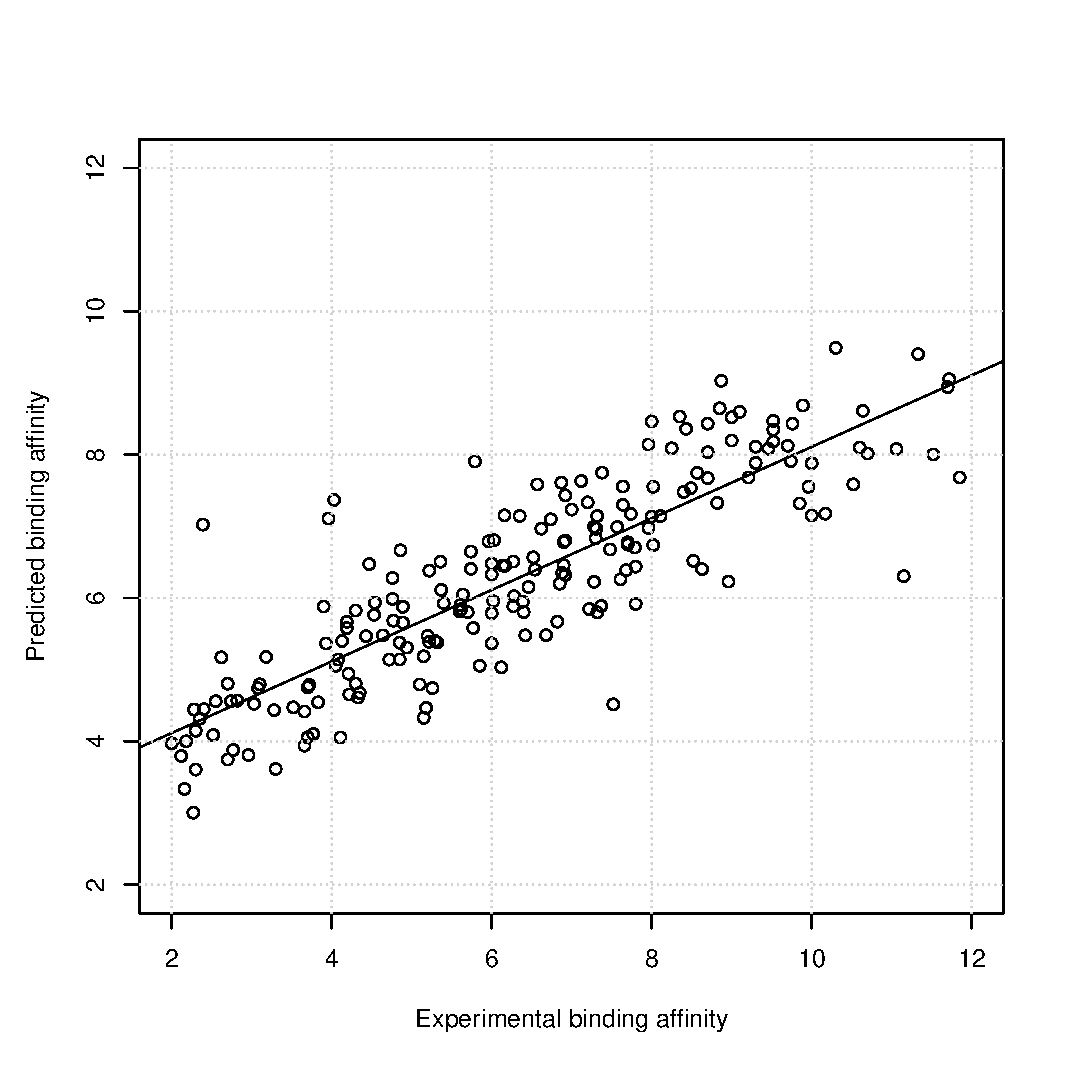
\includegraphics[width=4in]{pK-idockConf1RFScore.eps}
\end{center}
\caption{
{\bf Scatter plot of predicted binding affinity of docked pose against experimental binding affinity on PDBbind v2012 core set ($N$ = 201).} $R_p$ = 0.855, $R_s$ = 0.859, $RMSE$ = 1.41, $SD$ = 1.42.
}
\label{pK-idockConf1RFScore}
\end{figure}

\section*{Tables}

\begin{table}[!ht]
\caption{
\bf{Comparison of 21 scoring functions on PDBbind v2007 core set ($N$ = 195)}}
\begin{tabular}{lrrr}
\hline
Scoring function & $R_p$ & $R_s$ & $SD$\\
\hline
RF-Score & 0.774 & 0.762 & 1.59\\
ID-Score & 0.753 & 0.779 & 1.63\\
SVR-Score & 0.726 & 0.739 & 1.70\\
X-Score::HMScore & 0.644 & 0.705 & 1.83\\
AutoDock Vina & 0.570 & 0.612 & 2.18\\
DrugScoreCSD & 0.569 & 0.627 & 1.96\\
idock & 0.561 & 0.613 & 2.19\\
SYBYL::ChemScore & 0.555 & 0.585 & 1.98\\
DS::PLP1 & 0.545 & 0.588 & 2.00\\
GOLD::ASP & 0.534 & 0.577 & 2.02\\
SYBYL::G-Score & 0.492 & 0.536 & 2.08\\
DS::LUDI3 & 0.487 & 0.478 & 2.09\\
DS::LigScore2 & 0.464 & 0.507 & 2.12\\
GlideScore-XP & 0.457 & 0.435 & 2.14\\
DS::PMF & 0.445 & 0.448 & 2.14\\
GOLD::ChemScore & 0.441 & 0.452 & 2.15\\
SYBYL::D-Score & 0.392 & 0.447 & 2.19\\
DS::Jain & 0.316 & 0.346 & 2.24\\
GOLD::GoldScore & 0.295 & 0.322 & 2.29\\
SYBYL::PMF-Score & 0.268 & 0.273 & 2.29\\
SYBYL::F-Score & 0.216 & 0.243 & 2.35\\
\end{tabular}
\begin{flushleft}\label{ScoringFunctionComparison} Pearson's correlation coefficient $R_p$, Spearman's correlation coefficient $R_s$ and standard deviation $SD$ of the difference between predicted and experimental binding affinity on PDBbind v2007 core set ($N$ = 195). Scoring functions are sorted in the descending order of $R_p$. RF-Score, AutoDock Vina and idock rank 1st, 5th and 7th respectively in terms of Pearson's correlation coefficient.
\end{flushleft}
\end{table}

\begin{table}[!ht]
\caption{
\bf{Redocking success rates}}
\begin{tabular}{lrrrrrr}
\hline
& \multicolumn{2}{c}{PDBbind v2012} & \multicolumn{2}{c}{PDBbind v2011} & \multicolumn{2}{c}{CSAR NRC HiQ}\\
Condition & idock & Vina & idock & Vina & idock & Vina\\
\hline
$RMSD_1$ = $RMSD_m$ & 49\% & 53\% & 47\% & 54\% & 57\% & 71\%\\
$RMSD_2$ = $RMSD_m$ & 15\% & 16\% & 16\% & 14\% & 17\% & 13\%\\
$RMSD_3$ = $RMSD_m$ &  8\% &  7\% &  8\% &  8\% &  7\% &  4\%\\
$RMSD_4$ = $RMSD_m$ &  6\% &  6\% &  6\% &  5\% &  5\% &  3\%\\
$RMSD_5$ = $RMSD_m$ &  5\% &  4\% &  5\% &  5\% &  4\% &  1\%\\
$RMSD_6$ = $RMSD_m$ &  5\% &  3\% &  5\% &  4\% &  3\% &  3\%\\
$RMSD_7$ = $RMSD_m$ &  4\% &  4\% &  5\% &  4\% &  1\% &  2\%\\
$RMSD_8$ = $RMSD_m$ &  5\% &  3\% &  4\% &  3\% &  3\% &  2\%\\
$RMSD_9$ = $RMSD_m$ &  4\% &  3\% &  4\% &  3\% &  3\% &  2\%\\
\noalign{\smallskip}
$RMSD_1$ \textless\ 0.5 \AA & 10\% & 12\% & 11\% & 12\% & 21\% & 21\%\\
$RMSD_1$ \textless\ 1.0 \AA & 26\% & 31\% & 29\% & 31\% & 40\% & 47\%\\
$RMSD_1$ \textless\ 1.5 \AA & 43\% & 47\% & 45\% & 47\% & 61\% & 67\%\\
$RMSD_1$ \textless\ 2.0 \AA & 51\% & 56\% & 53\% & 56\% & 68\% & 73\%\\
$RMSD_1$ \textless\ 2.5 \AA & 56\% & 61\% & 58\% & 61\% & 72\% & 76\%\\
\noalign{\smallskip}
$RMSD_m$ \textless\ 0.5 \AA & 12\% & 15\% & 14\% & 15\% & 24\% & 26\%\\
$RMSD_m$ \textless\ 1.0 \AA & 35\% & 40\% & 39\% & 40\% & 54\% & 55\%\\
$RMSD_m$ \textless\ 1.5 \AA & 61\% & 65\% & 64\% & 65\% & 78\% & 84\%\\
$RMSD_m$ \textless\ 2.0 \AA & 72\% & 79\% & 74\% & 78\% & 86\% & 92\%\\
$RMSD_m$ \textless\ 2.5 \AA & 77\% & 85\% & 79\% & 84\% & 90\% & 94\%\\
\end{tabular}
\begin{flushleft}\label{SuccessRate} Redocking success rates of idock and AutoDock Vina on the PDBbind v2012 refined set ($N$ = 2,897), the PDBbind v2011 refined set ($N$ = 2,455), and the CSAR NRC HiQ Set 24Sept2010 ($N$ = 343) under various conditions regarding the $RMSD$ (Root Mean Square Deviation) values between the crystal and docked conformations. By default, both programs output 9 predicted conformations per ligand. $RMSD_i (i = 1,2,...,9)$ refers to the $RMSD$ value between the crystal conformation and the $i$th docked conformation, i.e. the one with the $i$th highest predicted binding affinity, while $RMSD_m$ refers to the $RMSD$ value between the crystal conformation and the closest docked conformation, i.e. the one with the minimum $RMSD$ value. $RMSD_m = \displaystyle\min_{i}RMSD_i\ (i = 1,2,...,9)$. In conclusion, idock has a slightly higher pose generation error than AutoDock Vina.
\end{flushleft}
\end{table}

\begin{table}[!ht]
\caption{
\bf{Virtual screening execution time}}
\begin{tabular}{lrrrrrr}
\hline
& \multicolumn{2}{c}{200-300g/mol} & \multicolumn{2}{c}{300-400g/mol} & \multicolumn{2}{c}{400-500g/mol}\\
& CPU & Elapsed & CPU & Elapsed & CPU & Elapsed\\
\hline
\multicolumn{7}{l}{\textbf{1HCL} human cyclin-dependent kinase 2}\\
Vina  & 12.57 &  3.33 & 22.55 &  5.91 & 51.62 & 13.41\\
idock &  0.63 &  0.16 &  0.92 &  0.24 &  1.38 &  0.36\\
\multicolumn{7}{l}{\textbf{1J1B} human tau protein kinase I}\\
Vina  &  9.07 &  2.47 & 14.69 &  3.92 & 32.28 &  8.49\\
idock &  0.78 &  0.21 &  1.25 &  0.33 &  2.35 &  0.62\\
\multicolumn{7}{l}{\textbf{1LI4} human S-adenosylhomocysteine hydrolase}\\
Vina  & 11.82 &  3.30 & 19.08 &  5.22 & 39.41 & 10.64\\
idock &  0.89 &  0.23 &  1.55 &  0.40 &  3.15 &  0.82\\
\multicolumn{7}{l}{\textbf{1V9U} human rhinovirus 2 coat protein VP1}\\
Vina  &  9.80 &  2.95 & 15.55 &  4.62 & 29.75 &  8.49\\
idock &  0.97 &  0.25 &  1.64 &  0.42 &  3.42 &  0.89\\
\multicolumn{7}{l}{\textbf{2IQH} influenza A virus nucleoprotein NP}\\
Vina  &  9.51 &  2.66 & 15.03 &  4.08 & 29.64 &  7.83\\
idock &  0.92 &  0.24 &  1.59 &  0.41 &  3.41 &  0.88\\
\multicolumn{7}{l}{\textbf{2XSK} Escherichia coli curli protein CsgC - SeCys}\\
Vina  & 10.44 &  2.71 & 17.89 &  4.61 & 40.58 & 10.41\\
idock &  0.71 &  0.19 &  1.16 &  0.30 &  2.16 &  0.56\\
\multicolumn{7}{l}{\textbf{2ZD1} HIV-1 reverse transcriptase}\\
Vina  &  9.78 &  2.70 & 17.67 &  4.76 & 42.03 & 11.33\\
idock &  0.97 &  0.25 &  1.52 &  0.39 &  2.60 &  0.69\\
\multicolumn{7}{l}{\textbf{2ZNL} influenza virus RNA polymerase subunit PA}\\
Vina  &  9.49 &  2.60 & 15.04 &  4.01 & 29.97 &  7.82\\
idock &  0.89 &  0.23 &  1.56 &  0.40 &  3.41 &  0.87\\
\multicolumn{7}{l}{\textbf{3BGS} human purine nucleoside phosphorylase}\\
Vina  &  9.59 &  2.57 & 16.50 &  4.37 & 38.42 & 10.14\\
idock &  0.95 &  0.25 &  1.55 &  0.40 &  2.81 &  0.74\\
\multicolumn{7}{l}{\textbf{3H0W} human S-adenosylmethionine decarboxylase}\\
Vina  &  9.85 &  2.64 & 17.67 &  4.70 & 41.69 & 11.04\\
idock &  0.88 &  0.23 &  1.35 &  0.35 &  2.20 &  0.58\\
\multicolumn{7}{l}{\textbf{3IAR} human adenosine deaminase}\\
Vina  & 11.25 &  3.03 & 20.21 &  5.39 & 46.93 & 12.53\\
idock &  0.80 &  0.21 &  1.21 &  0.32 &  2.01 &  0.53\\
\multicolumn{7}{l}{\textbf{3KFN} HIV protease}\\
Vina  & 10.53 &  2.80 & 18.37 &  4.83 & 42.43 & 11.03\\
idock &  0.77 &  0.20 &  1.20 &  0.32 &  2.09 &  0.55\\
\multicolumn{7}{l}{\textbf{Average across the above 12 receptors}}\\
Vina  & 10.31 &  2.81 & 17.52 &  4.70 & 38.73 & 10.26\\
idock &  0.85 &  0.22 &  1.38 &  0.36 &  2.58 &  0.67\\
\end{tabular}
\begin{flushleft}\label{ExecutionTime} CPU time and elapsed time in hours of docking 3,000 clean ligands of 3 molecular weight sets against 12 diverse receptors by AutoDock Vina and idock. idock outperforms AutoDock Vina by at least 8.69 times and at most 37.51 times.
\end{flushleft}
\end{table}

\end{document}
